%% 
%% Copyright 2019-2024 Elsevier Ltd
%% 
%% Version 2.4
%% 
%% This file is part of the 'CAS Bundle'.
%% --------------------------------------
%% 
%% It may be distributed under the conditions of the LaTeX Project Public
%% License, either version 1.2 of this license or (at your option) any
%% later version.  The latest version of this license is in
%%    http://www.latex-project.org/lppl.txt
%% and version 1.2 or later is part of all distributions of LaTeX
%% version 1999/12/01 or later.
%% 
%% The list of all files belonging to the 'CAS Bundle' is
%% given in the file `manifest.txt'.
%% 
%% Template article for cas-dc documentclass for 
%% double column output.

%\documentclass[a4paper,fleqn,longmktitle]{cas-dc}
\documentclass[a4paper,fleqn]{cas-dc}

%\usepackage[authoryear,longnamesfirst]{natbib}
%\usepackage[authoryear]{natbib}
\usepackage[numbers]{natbib}
\usepackage{enumitem}
\usepackage{listings}
\usepackage{xcolor}

% Custom styling for JSON code blocks
\definecolor{eclipseStrings}{RGB}{42,0,255}
\definecolor{eclipseKeywords}{RGB}{127,0,85}
\definecolor{jsonNumbers}{RGB}{128,0,0}

\lstdefinelanguage{json}{
    basicstyle=\small\ttfamily,
    stringstyle=\color{eclipseStrings},
    keywordstyle=\color{eclipseKeywords},
    commentstyle=\color{gray},
    numbers=left,
    numberstyle=\tiny\color{gray},
    stepnumber=1,
    numbersep=8pt,
    showstringspaces=false,
    breaklines=true,
    string=[s]{"}{"},
    literate=
     *{0}{{{\color{jsonNumbers}0}}}{1}
      {1}{{{\color{jsonNumbers}1}}}{1}
      {2}{{{\color{jsonNumbers}2}}}{1}
      {3}{{{\color{jsonNumbers}3}}}{1}
      {4}{{{\color{jsonNumbers}4}}}{1}
      {5}{{{\color{jsonNumbers}5}}}{1}
      {6}{{{\color{jsonNumbers}6}}}{1}
      {7}{{{\color{jsonNumbers}7}}}{1}
      {8}{{{\color{jsonNumbers}8}}}{1}
      {9}{{{\color{jsonNumbers}9}}}{1},
}
\newlist{todolist}{itemize}{2}
\setlist[todolist]{label=$\square$}

%%%Author definitions
\def\tsc#1{\csdef{#1}{\textsc{\lowercase{#1}}\xspace}}
\tsc{WGM}
\tsc{QE}
\tsc{EP}
\tsc{PMS}
\tsc{BEC}
\tsc{DE}
%%%
\input{reviewing}

\begin{document}
\let\WriteBookmarks\relax
\def\floatpagepagefraction{1}
\def\textpagefraction{.001}
\shorttitle{SolidSessionBench: Realistic Query Sequences}
\shortauthors{Ruben Eschauzier and Ruben Taelman}

\title[mode = title]{\todo{Change title to reflect intro changes}SolidSessionBench: Realistic Query Sequences for User-Oriented Decentralized Environments}                      

% \tnotetext[1]{This document is the results of the research
%    project funded by the National Science Foundation.}



\author[1]{Ruben Eschauzier}[orcid=0000-0001-0000-0000]
\cormark[1]
\ead{ruben.eschauzier@gmail.com}

\credit{TODO:}

%\address[1]{, Street 129, 1043 NX Amsterdam, The Netherlands}
\affiliation[1]{organization={Department of Electronics and Information Systems, Ghent University – imec},
                addressline={Universiteitstraat 4}, 
                city={Ghent},
%               citysep={}, % Uncomment if no comma needed between city and postcode
                postcode={9000}, 
                state={Flanders},
                country={Belgium}}

\author[1]{Ruben Taelman}[orcid=0000-0001-5118-256X]
\ead{ruben.taelman@ugent.be}
\ead[url]{www.rubensworks.net}


\credit{TODO:}

\begin{abstract}
% Context:      Why the need is so pressing or important
Emerging decentralized architectures give users complete control over their own data, 
scattering information across heterogeneous sources. 
Without a central authority to enforce consistency, users freely publish overlapping and conflicting claims, 
generating a highly multi-perspective environment. 
While client-side query engines can dynamically fetch and reconcile this information,
optimizing execution remains challenging due to a lack of prior knowledge regarding data distribution. 
By exploiting access patterns across repeated user query sequences, engines can overcome this knowledge gap.
% Need:         Why something needed to be done at all
However, accurately evaluating these personalized optimizations is difficult. 
Public query logs for decentralized environments are scarce, and existing benchmarks rely on static, 
template-based structures that fail to capture realistic behavioral variability.
% Task:         What was undertaken to address the need
To fill this gap, we introduce an evidence-based simulation 
of client query usage patterns as a reusable benchmark enabling 
realistic and reproducible evaluation of client-side optimization techniques.
% Object:       What the present document does or covers
We demonstrate its utility by evaluating client-side caching strategies 
for link traversal query processing.
By comparing our sequence-based approach against traditional, non-sequence-based workloads, 
we highlight how realistic sequence simulation heavily influences performance evaluations.
% Findings:     What the work done yielded or revealed
Ultimately, our benchmark reveals important performance dynamics, such as the impact 
of session switching and query refinement, that traditional workloads do not.
% Conclusion: What the findings mean for the audience
We conclude that modeling realistic user interactions provides an essential foundation 
for accurately evaluating client-side optimization techniques in decentralized environments.

\verb+\begin{keyword}+ \verb+...+ \verb+\end{keyword}+ 
which
contain the abstract and keywords respectively. 

\noindent Each keyword shall be separated by a \verb+\sep+ command.
\end{abstract}

\begin{graphicalabstract}

\includegraphics{figs/cas-grabs.pdf}
\end{graphicalabstract}

\begin{highlights}
\item Research highlights item 1
\item Research highlights item 2
\item Research highlights item 3
\end{highlights}

\begin{keywords}
quadrupole exciton \sep polariton \sep \WGM \sep \BEC
\end{keywords}


\maketitle


\section{Introduction}
\todo{Adjust to be more benchmarky}
Emerging web applications increasingly rely on decentralized architectures to give users control over their personal data.
Structured decentralized ecosystems, such as Solid~\cite{sambra2016solid} and Mastodon~\cite{raman2019challenges},
encourage users to keep their data in small, independent stores following shared data models.
This paradigm shift is increasingly vital for automated systems, such as LLM-based AI agents,
which query these decentralized structures to extract facts for task performance or question answering~\cite{walter2025grasp,karki2026agentic,bernerslee2017charlie}.
While this approach strengthens user autonomy, the absence of a central data authority naturally creates a highly multi-perspective environment. 
Data spreads across thousands of heterogeneous sources that frequently contain overlapping, diverse, 
or potentially conflicting claims.
Query engines must therefore dynamically fetch and integrate this information at runtime~\cite{taelman_sigweb_queryengineshypermedia_2024}, 
not only to discover conflicting statements and multiple perspectives, 
but to reconcile these claims to provide a coherent answer to the user or agent.

Traditional federated querying approaches~\cite{schwarte2011fedx,schmidt2011fedbench,heling2022federated} support the integration of decentralized data sources,
but they typically assume a small (10-100) set of well-described and consistently available endpoints~\cite{dang2023fedshop}. 
These assumptions fail once data is spread across thousands of small units that enforce local access-control policies.
In addition, enforcing fine-grained access control policies~\cite{esteves2021odrl} on large sources with expressive interfaces introduces notable 
overhead~\cite{padia2015attribute}, making standard approaches unsuitable for highly decentralized environments.

Newer decentralized environments, such as Solid, often expose data as lightweight HTTP resources instead of highly expressive query interfaces. 
Many of these resources are not known in advance and can only be discovered during query execution. 
While their simplicity lowers the cost of enforcing fine-grained controls,
this setting requires a federation model that can operate over a very large number of small sources,
many of which may be encountered at runtime, without relying on prior aggregation.
Traditional federated approaches are insufficient in this setting due to the assumption of a small number of large endpoints.
Additionally, these approaches often assume prior knowledge of the sources, which is not feasible in decentralized environments where discovery is a key requirement.
Executing SPARQL queries using Link Traversal-based Query Processing (LTQP)~\cite{hartig2009executing} fits these needs.
It discovers documents incrementally by following URIs encountered during execution, 
starting from an initial set of seed documents provided by either the user or the query.
Its link-driven, asynchronous traversal supports fine-grained permissions 
and allows systems to discover without knowing the location of all decentralized data sources beforehand.

However, the fact that LTQP discovers documents incrementally creates significant challenges for efficient execution. 
Using the traditional optimize-then-execute query processing paradigm is difficult, as the query itself determines which data will be accessed. 
As a result, the optimizer has no prior knowledge of the relevant data until the query’s traversal has already begun.
Some approaches optimize query execution without prior knowledge by using zero-knowledge query planning~\cite{hartig2011zero} or adaptive query processing~\cite{hanski2025link}. 
These yield modest but inconsistent performance gains, depending on the decentralized environment and the heuristics used~\cite{taelman2023link}.
However, other aspects of zero-knowledge LTQP optimization, such as link prioritization~\cite{hartig2016walking},
are unlikely to improve query result arrival times in emerging decentralized environments~\cite{eschauzier2025revisiting}.

Consequently, other works explore using precomputed server-side information as prior knowledge 
or relevance indexes to efficiently execute LTQP queries \newline \cite{tam2024opportunities,umbrich2011comparing,hanski2024observations}.
While these approaches offer greater performance benefits, they require the server to maintain these indexes.
This raises the cost of serving resources and complicates privacy and access control.

To avoid server-side overhead, engines can derive prior knowledge directly on the client.
In decentralized settings, LTQP operates inherently client-side, with a single engine instance serving one or more applications,
often specific to a particular user.
As these users and thus the used applications issue sequences of correlated queries,
the engine identifies frequently accessed data and its characteristics.
This allows engines to implement \emph{personalized} query optimization algorithms 
that leverage local access patterns to build necessary prior knowledge.


\begin{figure}
	\centering
	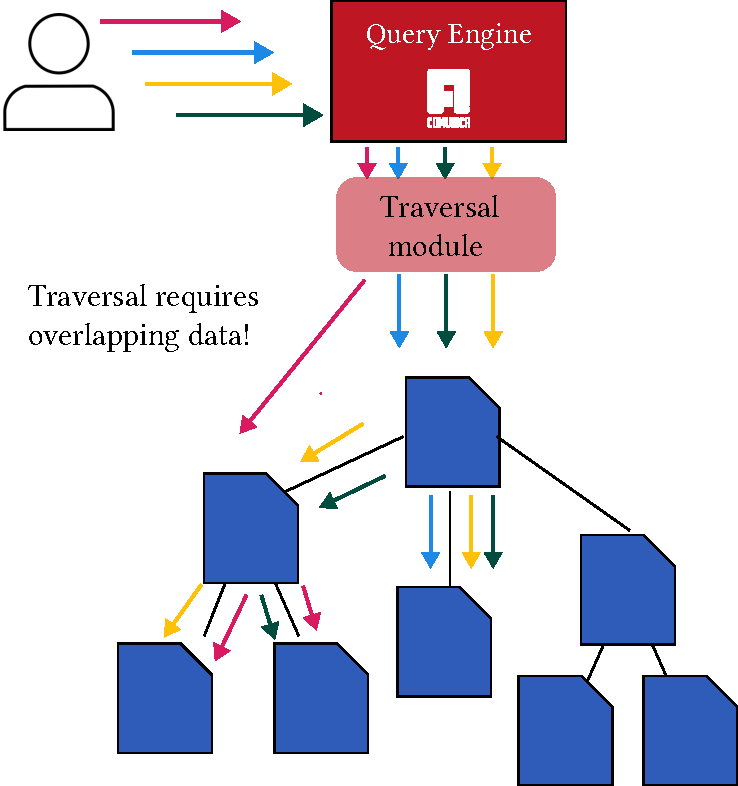
\includegraphics[width=.9\columnwidth]{figures/overlapping_queries_fixed.pdf}
	\caption{When users interact with query engines, their queries intentions and thus relevant data to the query can overlap, leading to opportunities for personalized optimization.}
	\label{fig:intro-overlap}
\end{figure}

Benchmarking these approaches requires realistic query sequences.
Traditional benchmarks (e.g., WatDiv~\cite{alucc2014diversified}, \\ BSBM~\cite{bizer2011berlin}, LargeRDFBench~\cite{saleem2018largerdfbench})
execute isolated or repeated query templates, which fails to capture client-side dynamics accurately. 
Furthermore, while centralized SPARQL optimization relies on
real query logs~\cite{berendt2013usewod2013,picalausa_what_2011,bonifati_darql_2018,stadler2024lsq}, 
such logs do not yet exist for decentralized LTQP environments. 
Consequently, we need a standardized benchmark that realistically simulates user query sequences 
to prevent fragmented evaluation practices.

In this paper, we address this gap by introducing SolidSessionBench,
a benchmark extending SolidBench~\cite{taelman2023link} to generate realistic query sequences.
These sequences capture usage patterns identified in social network literature, 
a domain naturally rich in multi-perspective data, 
alongside patterns observed in real-world SPARQL logs.

To evaluate the realism of our generated query sequences without access to real-world query logs, 
we investigate four baseline client-side caching strategies combined with two cardinality estimatoin techniques
in the Comunica LTQP engine~\cite{taelman2018comunica,taelman2023link}. 
We use these simple algorithms to establish a performance baseline and demonstrate the necessity of sequence-based evaluation.
Comparing this baseline against existing literature shows 
that current evaluation techniques are insufficient for client-side caching in LTQP.

By enabling researchers to evaluate personalized query optimization against actual user behaviors,
SolidSessionBench lays the foundation for performant client-side querying. 
Ultimately, efficient LTQP execution over decentralized sources facilitates the rapid identification of conflicting information
and the application of consistency fixes across multi-dimensional knowledge graphs.

In summary, this paper makes the following contributions:
\begin{itemize}
    \item We review empirical usage patterns in web and query-based systems
    to establish a foundation for realistic sequence simulation.
    
    \item We propose a simulation methodology based on the literature review
	 that models logical query sessions,
    user interest-driven data locality, and dynamic query refinements
    mapped to query engine choke points.
    
    \item We introduce SolidSessionBench, a fully configurable benchmark
    integrating this methodology to evaluate client-side query optimization
    under realistic conditions.
    
    \item We implement four baseline client-side caching strategies
    for Link Traversal Query Processing (LTQP),
    alongside two cache-based cardinality estimation techniques.
    
    \item We evaluate these strategies, demonstrating that realistic query sequences
    reveal critical performance dynamics that traditional benchmarking approaches miss.
\end{itemize}


This article extends our previous work presented at the International Semantic Web Conference 
(ISWC) 2026~\cite{eschauzier2026solidsessionbench}. 
While the initial study introduced the SolidSessionBench methodology and evaluated standard in-memory caching strategies, 
this version expands both the technical implementations and the experimental analysis. 

Specifically, we introduce in-memory and disk-based quad store caches to unify cached triple indexes. 
Furthermore, we enhance the original cache-based cardinality estimation technique
by incorporating reachability to generate more accurate estimates. 
Finally, we expand the experimental analysis by applying a linear mixed-effects regression model to quantify
the performance impact of individual query execution choke points. 

Beyond expanded explanations and examples, this extended version provides a thorough investigation of diverse cache implementations. 
Overall, we place a stronger focus on cache performance, the implications of our findings, 
and concrete directions for future research.

The remainder of this paper is structured as follows.
Section~\ref{sec:related-work} reviews prior benchmarking approaches and real-world query usage patterns.
Section~\ref{sec:simulation-methodology} outlines our simulation methodology and defines the resulting hyperparameters.
Section~\ref{sec:client-side-caching} introduces the technical mechanics of client-side caching strategies in LTQP.
Section~\ref{sec:evaluation} evaluates the benchmark using proxy measures of realism. 
Finally, Section~\ref{sec:conclusion} concludes the paper and presents a plan for benchmark sustainability.


\section{Literature Review}
\label{sec:related-work}
To ground our benchmark design in existing research and ensure a realistic sequence generator, 
this section reviews prior benchmarking approaches for client-side query optimization and real-world query usage patterns.

\subsection{Existing Benchmarking Approaches}
For the evaluation of client-side benchmarking techniques that rely on previous queries,
we primarily investigate caching literature, as this is a well-studied problem relevant to our work.

In the literature, we find three distinct benchmarking approaches: 
simulated micro benchmarks, simulated end-to-end query benchmarks, and real-world query logs.

% Existing evaluation methods for client-side query optimization 
% generally fall into three categories:


\textbf{Simulated micro benchmarks} attempt to isolate performance gains of the benchmarked approaches by fixing certain aspects of query execution.
This can range from fixing the cached data size~\cite{hartig2011caching} to controlling the percentage of query-relevant data present in the cache \cite{nicholson2024hpcache}. Fixing aspects of query execution makes it easier to isolate and understand the effect of specific caching mechanisms. 
However, it also gives an incomplete picture, because we don’t know how those fixed conditions relate to real workloads or how the methods perform when those assumptions don’t hold.

\textbf{Simulated end-to-end query benchmarks} use generated query sequences to evaluate performance. 
They aim to measure cache hit rate and overall execution behavior under the assumption that the simulated sequences reflect realistic usage.
In practice, the simulation is usually built by extending an existing benchmark so that it generates sequences instead of isolated queries. 
The sequence order is often determined by simple rules or by random selection.

A common approach is to use queries from existing benchmarks such as the Star Schema Benchmark \cite{o2009star} or the Berlin SPARQL Benchmark~\cite{bizer2011berlin}.
These queries are then randomly divided into sequences \cite{hartig2011caching,nicholson2024hpcache,folz2016cyclades}, with each sequence executed using a shared cache. This approach is straightforward but not realistic.
Prior work shows that real workloads contain user behavior patterns and temporal locality, and these patterns can be exploited by caching methods.
Random sequences fail to capture these properties.

More realistic is to adjust the query generators of existing benchmarks to include patterns in the query sequences.
Some works~\cite{williams2011enabling,martin2010improving} use a Pareto distribution to decide what entity is used to instantiate a query template.
This follows from the observation that many human activities follow a Pareto distribution~\cite{arnold2014pareto},
 with many queries relating to a small portion of the entities.

A third approach uses simulated query sequences that reflect the access patterns of specific applications.
One example is a workload that models data scientists exploring different aspects of the same entity—such as an author in a scholarly network—through consecutive, thematically related queries~\cite{chatzopoulos2022atrapos}.
Such simulations often include multiple query sessions, with new sessions beginning according to a probability parameter $p$.
Another example is a simulated application scenario focused on retrieving information about vacation destinations, which is used to assess caching effectiveness~\cite{martin2010improving}.

\textbf{Real-world query logs} Whenever available, query logs from actual applications form a highly relevant benchmarking approach.
However, obtaining these query logs can be challenging.
For SPARQL query optimization, query logs for a variety of endpoints are available, such as DBpedia~\cite{saleem2015lsq,stadler2024lsq,berendt2013usewod2013} and Wikidata~\cite{stadler2024lsq}.
These logs are extensively used in benchmarking SPARQL-based approaches~\cite{zhang2016secf,papailiou2015graph,lorey2013caching}.

The evaluation of personalized LTQP optimization would ideally use real-world query logs, but such logs do not exist.
To avoid the fragmented evaluation practices of current simulated approaches, the next best option is a unified simulated benchmark. 
A shared benchmark would provide a common basis for comparison, improve reproducibility, and prevent each paper from recreating its own evaluation setup.

\subsection{Real-world Query Usage Patterns}
\label{sec:related_work_qup}
To inform the benchmark design on what patterns should be simulated, we will outline three relevant client query usage patterns observed in the literature. The relevance is determined for our social network application use case.

\textbf{User Interest-Based Query Behavior}
Work on social networks shows users form communities based on shared interests~\cite{mislove2007measurement,clark2007understanding,backstrom2006group,kalaitzakis2012evolution}. 
These networks exhibit power-law degree distributions, small-world structures, and scale-free properties. 
This topology creates a dense core of high-degree nodes that connect many smaller, strongly clustered groups~\cite{mislove2007measurement}. 
Simulation studies confirm that this interest-driven group formation is stable and reliably modeled~\cite{amblard2015models,hamill2009social}.

Furthermore, empirical research formally establishes that shared interests directly drive a higher degree of explicit and implicit interactions between users~\cite{mitzlaff2013user}. 
These findings justify our simulation of user-relatedness and interest-driven behavior when generating query sequences.

\textbf{Logical Query Sessions}
Analysis of web browsing behavior shows that activity is best grouped into \emph{logical sessions}: sequences of user interactions focused on specific goals, 
rather than purely time-bound intervals~\cite{meiss_whats_2009,sadagopan2008characterizing,schneider2009understanding}. 
These task-oriented sessions frequently involve non-linear navigation, 
including backtracking. 
New sessions begin in approximately $15\%$ of clicks, 
following a log-normal distribution with average size and depth means of 6.1 and 3, respectively. 

These patterns also appear in application navigation. 
In a decentralized social media application, for example, 
a user viewing a feed might click a creator's username, view comments, or like a post. 
Because the parameters of each new query derive directly from the preceding query's results, 
these queries chain together into structures mirroring logical web sessions. 
Additionally, direct searches for specific posts or topics reflect standard session-switching behavior. 

Consequently, interactive applications generate sequences of interdependent requests~\cite{vogele2018wessbas}. 
This dynamic informs the design of Facebook's TAO data store, 
which is explicitly optimized for workloads driven by the user's step-by-step traversal of the social graph within the interface~\cite{bronson2013tao}.

\textbf{Query Refinement}  
Analysis of SPARQL queries issued to the DBpedia endpoint reveals that 
users frequently submit related queries in streaks~\cite{bonifati2020analytical,zhang2020characterizing}. 
These streaks consist of query sequences that share an underlying intention but undergo 
iterative refinement to achieve the user's objective. 
Previous studies initially introduced the concept of SPARQL query sessions specifically to analyze 
robotic queries~\cite{zhang2020characterizing,bonifati2020analytical}.

In this benchmark, we focus on organic query sequences~\cite{zhang2020characterizing}, 
which users generate through interactions with software or browsers~\cite{malyshev2018getting}.
Because organic interactions are driven by application design rather than underlying data organization, 
we assume these user behaviors will also emerge in applications navigating structured decentralized environments
Furthermore, we deprioritize robotic queries because their sequences can 
already be simulated by traditional benchmark approaches~\cite{taelman2023link,bizer2011berlin,alucc2014diversified}.

For both organic and robotic queries, analysis of total usage and reformulations (removals and additions) 
of operators over all query logs shows that filter, union, and optional operators account for the vast majority of reformulated queries.

Recent analyses of Wikidata query logs further demonstrate that query development is an iterative process of design,
debugging, and maintenance~\cite{arenas2025exploring}.
Based on this empirical data, 
exploratory querying encompasses six core behaviors~\cite{arenas2025exploring}:
\textbf{result refinement} to reduce records via filters or selective triple patterns,
\textbf{result generalization} to retrieve more entities by broadening parameters,
such as adding superclasses or increasing limits,
\textbf{result extension} to fetch additional attributes by appending new triple patterns,
\textbf{bug fixing} to correct structural errors like invalid URIs,
\textbf{query refinement} to adjust complex language features,
and \textbf{shifting query intent} to pivot topics by altering core predicates.

These findings confirm that real-world querying relies on dynamic, step-by-step modifications rather than the static execution of independent templates.
Consequently, existing evaluation frameworks fail to capture how users actively interact with data systems. 
Evaluating system performance for these exploratory query sequences remains a critical research challenge, 
explicitly requiring new benchmarks to validate progress~\cite{arenas2025exploring}. 
Therefore, modeling these empirical sequence patterns is essential to accurately assess client-side 
query optimization techniques.
\section{Query Sequence Benchmark}
\label{sec:simulation-methodology}
In this section, we detail our simulation methodology and the resulting hyperparameters.
We base our sequence generator on SolidBench~\cite{taelman2023link}, 
which simulates realistic decentralized social media applications within the Solid ecosystem.
SolidBench utilizes the Social Network Benchmark (SNB) dataset~\cite{erling2015ldbc,angles2020ldbc} 
and applies the Linked Data Benchmark Council (LDBC) choke point methodology~\cite{angles2014linked}.

The choke point methodology is a benchmark design strategy that targets specific query execution 
and optimization bottlenecks in current database management systems~\cite{boncz2013tpc}.
Inspired by classical benchmarks like TPC-H, this approach uses these technical challenges to guide research and system development. 
For graph data, choke points include estimating cardinality during traversals with data skew, determining optimal join orders, 
and handling scattered index access patterns that lack predictable locality~\cite{erling2015ldbc}. 
In practice, a choke point-based benchmark design strategy first identifies critical execution challenges, 
then designs queries or modifications that explicitly test them.

We evaluate our prioritization algorithms using SolidBench~\cite{taelman2023link},
the state-of-the-art benchmark for structured decentralized environments.
SolidBench simulates a social network containing users, posts, and comments,
all described by a single ontology.
To represent Solid pods, the benchmark fragments data so that all information
related to a specific user resides in a single pod.
Under default settings, SolidBench generates 158,233 RDF files across
1,531 data vaults, totaling 3,556,159 triples.

To simulate a highly distributed network, SolidBench partitions the Social
Network Benchmark (SNB) dataset into individual data pods.
Its sequential architecture executes in four modular steps:
\begin{enumerate}
    \item The LDBC Datagen generates the underlying dataset.
    \item An enhancer creates additional data, such as noise triples that
    do not participate in queries.
    \item A dataset fragmenter partitions the triples into a Solid-like structure.
    \item The SPARQL queries are instantiated.
\end{enumerate}

The workload combines standard SNB \textit{interactive} queries (\textit{short} and \textit{complex})
with custom \textit{discover} templates that explicitly target
Link Traversal Query Processing (LTQP) choke points.
During execution, a client-side engine dynamically traverses links
between these scattered pods to resolve the queries.

To support sequence-based evaluation, we significantly extend and restructure three core SolidBench components:
\begin{itemize}
    \item \textbf{Query Generator:} Modified to produce correlated query sequences
    that reflect empirical usage patterns.
    \item \textbf{Dataset Generator:} Enhanced to model interest-based similarities
    among simulated users.
    \item \textbf{Benchmark Runner:} Updated with sequence execution logic to facilitate
    reproducible experiments and simplify the generation of default configuration files.
\end{itemize}

Link traversal engines cannot currently solve \textit{complex} queries in a feasible timeframe,
so we omit them from our default benchmark configuration.
However, because the sequence generator is fully configurable,
researchers can easily include complex query templates in future benchmarks
as traversal engines improve.


\subsection{Realism of Query Sequences}
To ensure SolidSessionBench accurately reflects user behavior in decentralized environments, 
we base our simulation methodology on the LDBC methodology used for data generation.
The sequence generator synthesizes empirical usage patterns established in Section~\ref{sec:related-work} to form a 
grounded simulation methodology that reflects real-world patterns.

Because direct, real-world query logs for highly decentralized LTQP environments do not currently exist,
we maintain and evaluate realism through a three-pillared approach:

\begin{itemize}
    \item \textbf{Topological Realism (User Interests):} We utilize the established LDBC social network topology
    to model explicit and implicit user relatedness, ensuring data access patterns mirror natural community formations 
    rather than uniform distributions. Due to the proven realism of the LDBC data generator~\cite{prat2014community}, 
    our simulations inherit this empirically proven structure.
    
    \item \textbf{Navigational Realism (Logical Sessions):} We restrict query sequences to directed dependency graphs.
    This simulates realistic ``click-through'' application navigation, 
    accounting for empirically observed session lengths and log-normal transition probabilities.  
 
    \item \textbf{Exploratory Realism (Query Refinement):} We replace static templates with dynamic query transformations. 
    Mapping real-world SPARQL refinements (e.g., result generalization, intent shifting) directly to execution choke points 
    ensures engines face realistic structural variability.
\end{itemize}

We evaluate the success of this simulation by measuring proxy variables such as
cache hit rates, execution times, and relatedness of relevant data accessed during queries. 
We then compare these outcomes against theoretical baselines and random sequence generation. 
This comparative evaluation demonstrates that our query sequence simulation captures essential 
performance dynamics that existing benchmarks miss.


\subsection{Simulation Methodology}
Our methodology models three interdependent behaviors: task-oriented logical sessions,
user interests for data locality,
and refinement patterns for iterative query development.

\subsubsection{Logical Query Sessions}
To model logical sessions, we categorize queries into four primary topics: 
person-specific messages, forum information, person attributes, and message attributes. 
Because queries in decentralized environments often depend on preceding results, 
we map the output types of each template to valid subsequent templates. 
This creates a directed graph of query progression that governs the flow of a logical session.
% \rt{If you can't add a figure in the introduction, I'd add one here, to illustrate what you explain in this paragraph.}

Within a session, a template's \emph{instantiation values} are typically derived 
from the previous query's results. 
To realistically simulate this ``click-through'' 
behavior, we execute centralized equivalents of the LDBC SNB queries using 
QLever~\cite{bast2017qlever}. 
We then randomly sample the returned result set 
to instantiate the subsequent query template. 
If a query yields no results, 
we fall back to our default, interest-based instantiation methodology.

As an example, consider the following data distributed across a 
decentralized environment:

\begin{lstlisting}[
    language=json,
    caption={(a) Alice's profile document (\url{https://pod.example/alice/profile.ttl}).},
    label={lst:example_dataset_alice_profile},
    breaklines=true,
    basicstyle=\small\ttfamily
]
<https://pod.example/alice/profile.ttl#me> a :Person ;
    :knows <https://pod.example/bob/profile.ttl#me> ;
    :hasInbox <https://pod.example/alice/inbox> .
\end{lstlisting}
\continuelisting

\begin{lstlisting}[
    language=json,
    caption={(b) Bob's profile document (\url{https://pod.example/bob/profile.ttl}).},
    label={lst:example_dataset_bob_profile},
    breaklines=true,
    basicstyle=\small\ttfamily
]
<https://pod.example/bob/profile.ttl#me> a :Person ;
    :posts <https://pod.example/bob/posts/1> .
\end{lstlisting}
\continuelisting

\begin{lstlisting}[
    language=json,
    caption={(c) Bob's post (\url{https://pod.example/bob/posts/1}).},
    label={lst:example_dataset_bob_post},
    breaklines=true,
    basicstyle=\small\ttfamily
]
<https://pod.example/bob/posts/1> a :Post ;
    :content "Hello Solid world!" .
\end{lstlisting}
\continuelisting

\begin{lstlisting}[
    language=json,
    caption={(d) Alice's interests document (\url{https://pod.example/alice/interests.ttl}).},
    label={lst:example_dataset_alice_interests},
    breaklines=true,
    basicstyle=\small\ttfamily
]
<https://pod.example/alice/profile.ttl#me> :interestedIn "Wildlife" .
\end{lstlisting}
\continuelisting

\begin{lstlisting}[
    language=json,
    caption={(e) Wildlife forum document (\url{https://pod.example/forum/wildlife.ttl}).},
    label={lst:example_dataset_forum_wildlife},
    breaklines=true,
    basicstyle=\small\ttfamily
]
<https://pod.example/forum/wildlife.ttl> a :Forum ;
    :hasPost <https://pod.example/ruben/posts/9> ;
    :hasComment <https://pod.example/bob/comment/1> ;
    :hasTopic "Wildlife" .
<https://pod.example/bob/comment/1> :responseTo <https://pod.example/ruben/posts/9> .
\end{lstlisting}

% \begin{lstlisting}[
%     language=json,
%     caption={A minimal decentralized dataset distributed across documents.},
%     label={lst:example_dataset},
%     breaklines=true,
%     basicstyle=\small\ttfamily
% ]
% @prefix : <https://example.org/voc#> .

% # File: https://pod.example/alice/profile.ttl
% <https://pod.example/alice/profile.ttl#me> a :Person ;
%     :knows <https://pod.example/bob/profile.ttl#me> ;
%     :hasInbox <https://pod.example/alice/inbox> .

% # File: https://pod.example/bob/profile.ttl
% <https://pod.example/bob/profile.ttl#me> a :Person ;
%     :posts <https://pod.example/bob/posts/1> .

% # File: https://pod.example/bob/posts/1
% <https://pod.example/bob/posts/1> a :Post ;
%     :content "Hello Solid world!" .

% # File: https://pod.example/alice/interests.ttl
% <https://pod.example/alice/profile.ttl#me> :interestedIn "Wildlife" .

% # File: https://pod.example/forum/wildlife.ttl
% <https://pod.example/forum/wildlife.ttl> a :Forum ;
%     :hasPost <https://pod.example/ruben/posts/9> ;
%     :hasComment <https://pod.example/bob/comment/1> ;
%     :hasTopic "Wildlife" .
% <https://pod.example/bob/comment/1> :responseTo <https://pod.example/ruben/posts/9> .
% \end{lstlisting}

The generator randomly selects a user and simulates
a realistic sequence of queries that reflects real-world user behavior.
Given 
Given this dataset, and two query 
templates: one to fetch a person's posts and another to retrieve the 
content of a specific post, the generator can create a query sequence, which can contain multiple
logical sessions.
For user ``alice'', we can start the sequence (and first logical session) by 
executing the first query template (Q1) to discover Bob's posts, 
as shown in Listing~\ref{lst:query_1}.

\begin{lstlisting}[
    language=SPARQL,
    caption={Initial query (Q1) fetching Bob's posts.},
    label={lst:query_1},
    breaklines=true,
    basicstyle=\small\ttfamily
]
SELECT ?post WHERE {
  <https://pod.example/bob/profile.ttl#me> :posts ?post .
}
\end{lstlisting}

The client-side query engine executes this query by traversing to Bob's 
profile document, returning the result binding: 
`?post = <https://pod.example/bob/posts/1>`.

To simulate a user clicking on this discovered post, the sequence 
generator instantiates the next query template dynamically. It extracts 
the value bound to ``?post'' from the results of Q1 and injects it as the 
subject of Q2, as shown in Listing~\ref{lst:query_2}.

\begin{lstlisting}[
    language=SPARQL,
    caption={Dynamic sequence query (Q2) instantiating a variable from Q1.},
    label={lst:query_2},
    breaklines=true,
    basicstyle=\small\ttfamily
]
SELECT ?content WHERE {
  <https://pod.example/bob/posts/1> :content ?content .
}
\end{lstlisting}

This example demonstrates that the instantiation of Q2 strictly depends 
on the execution results of Q1. Because Q2 requires an instantiated 
post URI from Q1, these queries are directionally dependent; reversing 
their order leaves the generator with no method to instantiate the 
initial query parameters. Consequently, structured logical query sequences 
naturally emerge from these interdependencies, accurately reflecting 
realistic exploratory user behavior.

Finally, we simulate logical session switching. 
Drawing from web browsing behavior, we assign each sequence a session-switching probability sampled from a log-normal 
distribution with a mean of 15\%~\cite{meiss_whats_2009,schneider2009understanding}. 
During sequence generation, a session switch triggers a random choice with equal probability: the engine either starts a new 
session (using interest-based instantiation) or resumes a previous one (deriving instantiation values from that session's last executed query).
To prevent repetitive queries and maintain a uniform distribution of template instantiations, 
we explicitly prohibit backtracking within our model. 
Additionally, we maintain a balanced template distribution by dynamically 
scaling down each template's selection probability proportionally to its 
overall frequency.

Continuing our running example, a session switch occurs after executing Q2. 
Instead of continuing sequence generation from the content of Bob's post, 
the generator terminates the current path and selects a new template to 
instantiate: a query for posts within a forum.

As shown in Listing~\ref{lst:query_3}, the generator selects a wildlife forum 
as the initial instantiation value. This query requires an entirely separate 
data path to execute, breaking the dependency chain of the previous queries 
and representing a clear change in user intent. We are still generating the same
\textit{query sequence}, but the session switch introduces a new \textit{logical session} within that sequence.

\begin{lstlisting}[
    language=json,
    caption={Independent query (Q3) initiating a session switch to explore a wildlife forum.},
    label={lst:query_3},
    breaklines=true,
    basicstyle=\small\ttfamily
]
SELECT ?post WHERE {
  <https://pod.example/forum/wildlife.ttl> :hasPost ?post .
}
\end{lstlisting}

\subsubsection{User Interest Modeling}

Individuals interact more frequently with users sharing similar interests~\cite{mitzlaff2013user}. 
To simulate this behavior, we use the underlying LDBC dataset utilized by SolidBench~\cite{erling2015ldbc}, 
which inherently models realistic user preferences. 
The LDBC generator, Datagen, produces person profiles containing specific interests, 
educational backgrounds, and workplaces. 
It links users based on these demographic and interest overlaps, 
yielding a non-random network topology with a realistic degree distribution.

We use this interest-driven topology to generate template instantiation values 
for the first query of each logical session. 
Specifically, we construct a binary feature vector $v_{k}$ for each user $k$:
\begin{equation}
 v_{k} = (x_{k,1}, \dots, x_{k,n}, y_{k,1}, \dots, y_{k,m}),
\end{equation}
where $x_{k,j}=1$ if user $k$ holds stated interest $j$, and $y_{k,m}=1$ 
if user $k$ completed study $m$.

For each sequence, we randomly select a base person $k$ and compute the cosine similarity 
between $v_{k}$ and the feature vectors of all other users.
Let $N$ be the total number of users. To maintain efficiency at large scale factors, 
we restrict our candidate pool to $C_{k,M}$, defined as the set of the top $M < N$ users 
ranked by similarity to $k$. 
Template instantiation values are then selected probabilistically using a softmax function 
with temperature $T$:

\begin{equation}
   P(i \mid k) = \frac{e^{s_{k,i} / T}}{\sum_{u \in C_{k,M}} e^{s_{k,u} / T}},
\end{equation}

where $s_{k,i}$ is the similarity score between base person $k$ and candidate $i \in C_{k,M}$. 
For templates requiring non-person values (e.g., posts or activities),
selection probabilities are derived from the similarity scores of the content's creators.

Continuing our running example, consider an expanded decentralized environment containing a
second forum dedicated to pottery, as shown in
Listing~\ref{lst:augmented_dataset} as well as all documents in Listing~\ref{lst:example_dataset_alice_interests}.

\begin{lstlisting}[
    language=json,
    caption={The additional pottery forum document (\url{https://pod.example/forum/pottery.ttl}).},
    label={lst:augmented_dataset},
    breaklines=true,
    basicstyle=\small\ttfamily
]
<https://pod.example/forum/pottery.ttl> a :Forum ;
    :hasTopic "Pottery" .
\end{lstlisting}

To determine what instantiation value to use for the forum query for user Alice, we construct 
binary feature vectors over a small global feature space: 
$\text{(Wildlife, Pottery)}$. 

Alice's profile states an explicit interest in `Wildlife', yielding vector 
$v_{\text{Alice}} = (1, 0)$. While the forums in the data have topic statements, thus
the vectors for the forums are $v_{\text{Wildlife}} = (1, 0)$ and
$v_{\text{Pottery}} = (0, 1)$. 

This gives us a cosine similarity of $s_{\text{Alice},\text{Wildlife}} = 1$ and
$s_{\text{Alice},\text{Pottery}} = 0$. Then using softmax with a temperature of $T = 0.5$,
we compute the selection probabilities for the two forums:

\begin{align*}
    P(\text{Wildlife} \mid \text{Alice}) = \frac{e^{1 / 0.5}}{e^{1 / 0.5} + e^{0 / 0.5}} \approx 0.88, \\
    P(\text{Pottery} \mid \text{Alice}) = \frac{e^{0 / 0.5}}{e^{1 / 0.5} + e^{0 / 0.5}} \approx 0.12.
\end{align*}

Consequently, when initiating or switching a session, the generator is more likely to select the
`Wildlife' forum for Alice, reflecting her interests.

\subsubsection{Refinement Patterns}

The benchmark simulates query refinement by applying 
composable transformations to an instantiated query template. 
Following our literature review, we focus on transformations 
(and their reciprocal counterparts) that add or modify 
BGPs, \texttt{OPTIONAL} clauses, \texttt{UNION} blocks, 
and query instantiation values.

To ensure these transformations meaningfully alter query execution 
rather than superficially appending triples, we apply a 
choke point-based design methodology~\cite{angles2014linked}. 
The generator sequentially applies refinements to a base 
SolidSessionBench template. By mapping empirical exploratory 
usage patterns~\cite{arenas2025exploring} to concrete 
planning (P) and traversal (T) choke points, we translate 
real-world user behaviors into rigorous execution bottlenecks 
for query engines.

The planning choke points, derived from empirical usage 
patterns~\cite{arenas2025exploring} and relevant LDBC 
choke points~\cite{angles2020ldbc}, are defined as follows:
\begin{enumerate}[label=\textbf{P.\arabic*}, leftmargin=*]
    \item Involves adding or 
    removing a \texttt{FILTER}, requiring prior knowledge 
    to adjust query plans and estimate selectivity.
    \item Addresses 
    adding or removing \texttt{UNION} or \texttt{OPTIONAL} 
    clauses to alter filter push-down capabilities and 
    complicate query planning.
    \item Covers adding 
    or removing selective triple patterns, forcing the engine 
    to identify changes and re-optimize the plan.
    \item Focuses 
    on adding or removing non-selective triple patterns.
\end{enumerate}

Beyond planning, these refinements introduce traversal 
choke points that expand upon those established in 
SolidBench~\cite{taelman2023link,taelman2023evaluation}:
\begin{enumerate}[label=\textbf{T.\arabic*}, leftmargin=*]
    \item Expands 
    or contracts the reachable sub-web through 
    predicate additions.
    \item Shifts the sub-web 
    by substituting the traversal starting point.
    \item Changes the number 
    of hops required to obtain relevant data, corresponding 
    to SolidBench choke points L.1--L.6~\cite{taelman2023evaluation}.
    \item Alters the usability of structural indexes, such as type indexes, 
    corresponding to SolidBench choke point 
    L.8~\cite{taelman2023evaluation}.
\end{enumerate}

These choke points directly map to the exploratory query 
behaviors identified in Section~\ref{sec:related_work_qup}:
\begin{itemize}[leftmargin=*]
    \item \textbf{Result refinement} corresponds to 
    P.1 and P.3, as it narrows results via \texttt{FILTER} 
    constraints and selective triple patterns.
    \item \textbf{Result generalization} corresponds to 
    P.3 and P.4, expanding existing BGPs with selective 
    or non-selective triple patterns.
    \item \textbf{Result extension} maps to P.2, P.3, 
    and P.4 by appending triple patterns to BGPs or 
    introducing \texttt{OPTIONAL} and \texttt{UNION} 
    blocks that alter filter push-down capabilities.
    \item \textbf{Shifting query intent} corresponds to 
    T.1 and T.2, substituting instantiation values to 
    initiate traversal from different seed documents, 
    thereby shifting or expanding the reachable sub-web.
    \item \textbf{Query refinement} maps to P.2, 
    modifying the structural complexity of the query 
    by adding or removing \texttt{OPTIONAL} and 
    \texttt{UNION} blocks.
\end{itemize}

Finally, the generator supports variable instantiation 
within refinements, allowing users to bind pattern variables 
to specific values randomly selected from configuration candidates. 
Users can define custom refinement patterns via JSON files to 
augment the default configurations. 

An example of a slimmed-down default configuration is 
provided in Listing~\ref{lst:refinement_config}. 
This entry specifies an \texttt{OPTIONAL} refinement 
pattern that appends a triple pattern to retrieve the 
messages liked by a person. 

The \texttt{location} parameter is set to 0, indicating 
that the triple pattern is added to the first existing 
\texttt{OPTIONAL} block, or to a new block if none is 
present. The default benchmark suite also includes a 
reciprocal configuration where \texttt{operation} is 
set to ``removal'', which instead deletes the triple pattern 
from the first \texttt{OPTIONAL} block.

\begin{lstlisting}[
    language=json,
    caption={Example configuration for an \texttt{OPTIONAL} refinement pattern.},
    label={lst:refinement_config},
    breaklines=true,
    basicstyle=\small\ttfamily,
    columns=fullflexible
]
{
  "type": "OPTIONAL",
  "id": 0,
  "operation": "addition",
  "description": "Add triple for likes (P.1, T.2)",
  "location": 0,
  "target": [
    {
      "subject": { 
        "value": "person", 
        "termType": "variable" 
      },
      "predicate": { 
        "value": ".../vocabulary/likes", 
        "termType": "namedNode" 
      },
      "object": { 
        "value": "likedMessage", 
        "termType": "variable" 
      }
    }
  ]
}
\end{lstlisting}

All defaults, along with 
complete documentation, are available on GitHub.%
\footnote{\url{https://github.com/SolidBench/SolidBench.js/tree/master/templates/refinements}}


\subsection{Hyperparameters}

The sequence generation process introduces several new hyperparameters, 
which are detailed in Table~\ref{tab:generation_hyperparameters} together with their default values. 
To guarantee reproducibility despite extensive random sampling, 
a single seeded pseudo-random number generator (PRNG) is used througout the 
entire pipeline.

\begin{table}[htbp]
    \centering
    \caption{LogT-normal distribution parameters ($\mu, \sigma$) control the queries per sequence, 
    queries per logical session, and the probability of switching logical sessions. 
    Refinement parameters define the likelihood (\texttt{patternProbability}) 
    and bounds (\texttt{min/maxRefinementLength}) of generating a refinement sequence for a given query. 
    Instantiation relies on a softmax \texttt{temperature} and a \texttt{maxLogits} 
    cutoff for similarity-based entity selection.}
    \label{tab:generation_hyperparameters}
    \begin{tabular}{l l c}
        \toprule
        \textbf{Category} & \textbf{Parameter} & \textbf{Value} \\
        \midrule
        \textbf{Distributions} ($\mu, \sigma$) 
        & \texttt{Sequence Length} & 3.0, 0.2 \\
        & \texttt{Session Length} & 1.7, 0.5 \\
        & \texttt{Transition Probability} & -2.0, 0.25 \\
        \addlinespace
        \textbf{Refinements} 
        & \texttt{patternProbability} & 0.1 \\
        & \texttt{min/maxRefinementLength} & 2, [3--5] \\
        \addlinespace
        \textbf{Instantiation} 
        & \texttt{temperature} & 0.1 \\
        & \texttt{maxLogits} & 5--10 \\
        \bottomrule
    \end{tabular}
\end{table}


\section{Caching in Link Traversal-based Query Processing}
\label{sec:client-side-caching}

Unlike traditional query engines that evaluate queries against a centralized, pre-built index, 
LTQP evaluates queries directly over the live Web~\cite{taelman2023evaluation,hartig2012sparql} 
using the ``follow-your-nose'' principle. 

Starting from a seed URI (often extracted from the query), 
the engine fetches data via a \emph{link queue} (governed by \emph{reachability criteria}~\cite{hartig2009executing}) 
and deposits the retrieved triples into an \emph{active local store}. 
This local store is an in-memory dataset over which the query executes, 
typically utilizing dictionary encoding~\cite{taelman2018comunica}. 

Previous work~\cite{hartig2011caching} established the fundamental concept of caching within this paradigm,
demonstrating that a local repository of recently accessed Web documents 
mitigates the high network latency inherent to LTQP.

For our experiments, we use the Comunica LTQP engine~\cite{taelman2018comunica,taelman2023link}. 
As a JavaScript-based engine, it relies on the event loop to asynchronously interleave HTTP requests during traversal and local query execution. 

We use caching-based algorithms to validate SolidSessionBench query sequences and compare them against alternative benchmarking methods in the literature.
Implementing these strategies establishes strong baselines for evaluating caching in traversal engines.
This section introduces four cache implementations, each storing dereferenced quads differently.
We also evaluate two cardinality estimation approaches that use cached quads to improve query planning and execution.
Because these estimates require an indexed cache, we omit them for the unindexed baseline.

\subsection{Cache Implementations}
\paragraph{Unindexed Cache}
This baseline caches raw triple arrays alongside source metadata.
On a cache hit, the engine retrieves and indexes these triples into the active local store.

\paragraph{Indexed Cache}
This approach pre-indexes triples and stores them in an in-memory LRU cache.
On a hit, the engine extracts only the triples matching the query patterns.
Combined with dictionary encoding, this pre-filtering reduces local store memory and indexing overhead,
potentially offsetting the higher initial ingestion costs.

\paragraph{Memory-based Quad store Cache}
\rt{The difference between indexed store and quad store is confusing. Could we call the first one just LRU Cache? I think that could solve it.}
This approach uses a quad store to unify cache indexes, saving memory and improving search efficiency.
The quad graph stores the source of the triples, allowing cache hits to retrieve data using an `?subject ?predicate ?object' query where the graph term matches the cached document's URL.

\paragraph{Disk-based Quad store Cache}
This approach stores the quad store on disk, providing the same advantages while supporting datasets larger than main memory.
We add a small in-memory cache for a `hot' subset of frequently accessed triples.
To make this memory cache scan-resistant, documents are only added if accessed multiple times.
This prevents long-running queries from evicting the entire cache.

\subsection{Cardinality Estimation Approaches}

Link traversal lacks prior knowledge regarding data distribution and availability, 
complicating query planning. 
We evaluate two cardinality estimation approaches using cached data to address this. 
\rt{I would make explicit here that you make the hypothesis that determining cardinalities using cached data is accurate enough for query planning}
The default Comunica cost-based optimizer~\cite{taelman2018comunica} uses these estimates to generate more accurate query plans,\rt{This is phrased in a confusing manner. Is this something that already exists? Or is it your contribution?}
replacing the zero-knowledge heuristics~\cite{hartig2011zero} traditionally used in link traversal.

\paragraph{Global Cache Cardinality Estimation}
This approach estimates cardinalities across the entire cache.
For each cache entry, it performs a query to count the number of matching triples 
and sums these counts to produce a final estimate.

\paragraph{Offline-traversal Cardinality Estimation}
Here, we store the outgoing links of each cached document.
For each query, we traverse the cache to find all documents reachable under the active reachability criterion,
to produce more accurate estimates by ignoring irrelevant data. 
If the seed document is missing from the cache, we fall back to the global cache estimation approach.

\rt{Regarding naming, what about "Reachability-agnostic Cache-based Cardinality Estimation" and "Reachability-aware Cache-based Cardinality Estimation"}


\subsection{Experimental Configurations}
For our experiments we evaluate three cache capacities: small (350k quads\rt{Let's use "triples"}, $\sim$10\% of the dataset), 
medium (700k, $\sim$20\%), and large (1.4M, $\sim$40\%). 
While the disk-based cache stores 1.4M quads on disk, 
and a a small in-memory cache of 25k, 50k, and 100k quads for the small, medium, and large configurations respectively.
% All cache implementations use the LRU eviction policy.

Our implementations adhere to the RFC-9111 specification~\cite{fielding2022rfc}, 
meaning the cache correctly interprets standard HTTP headers (e.g., Cache-Control) 
just like a web browser would. 
However, because the benchmark dataset is static, cache entries require no revalidation and never become stale. 
Consequently, observed hit rates are likely higher than in a live environment. 

Ultimately, comparing these strategies establishes $10$ baselines \rt{Can you explain how you get to 10?}
for caching performance in realistic user-centric environments, 
upon which future research into advanced caching approaches can build.
\section{Evaluation}
\label{sec:evaluation}
\todo{Improve naming algorithms to new names we selected}
\todo{Here outline also why we evaluate the benchmark this way, why this is a proxy for a useful benchmark
and then repeat again: no emperical data.}

We evaluate our benchmark using a scale 0.1 SolidBench dataset 
(158,233 RDF files, 1,531 vaults, 3,556,159 triples). 
Using the default hyperparameters in Table~\ref{tab:generation_hyperparameters}, 
we generate 8 sequences totaling 192 queries. 
These queries are from the interactive workload, are split into discover and short queries,
with multiple templates belonging to either of these groups.
Experiments run on an Ubuntu 20.04 machine (Intel Core i5-9400) 
with 16 GB RAM allocated to the engine and a 180-second query timeout. 
We repeat each sequence 10 times to minimize variance and 
inject a uniform 70–90 ms latency to simulate a realistic network environment.
The cache is scoped for a sequence, meaning no cache-state is shared between different executions or repetitions of
sequences.

% Outline the experimental setup, including machine scale and configurations. 
% State the primary aim: validating the benchmark. 
% Explain that validation relies on proxy metrics measuring data locality 
% (unique sources, cache hit rates, execution time) to demonstrate how 
% sequence design choices impact engine performance.
% Summarize our evaluation approach, which includes a holistic evaluation of benchmark characteristics, then
% a detailed analysis of logical session and interest modeling, refinement patterns, 
% and a comparison to alternative evaluation methods.

\subsection{Holistic Evaluation of Benchmark Characteristics}

First, we present the overall performance characteristics of the tested caching algorithms on the default configuration
of our introduced benchmark.

\paragraph{Unindexed LRU Cache}

In Figure~\ref{fig:unindexed-lru-cache-performance}, we find that the unindexed LRU cache reliably improves performance 
across all cache sizes, with larger caches yielding better results.
For total execution time of queries, the large cache is significantly better than the smaller cache sizes, while for
throughput the difference is less pronounced.

\begin{figure*}[t]
    \centering
    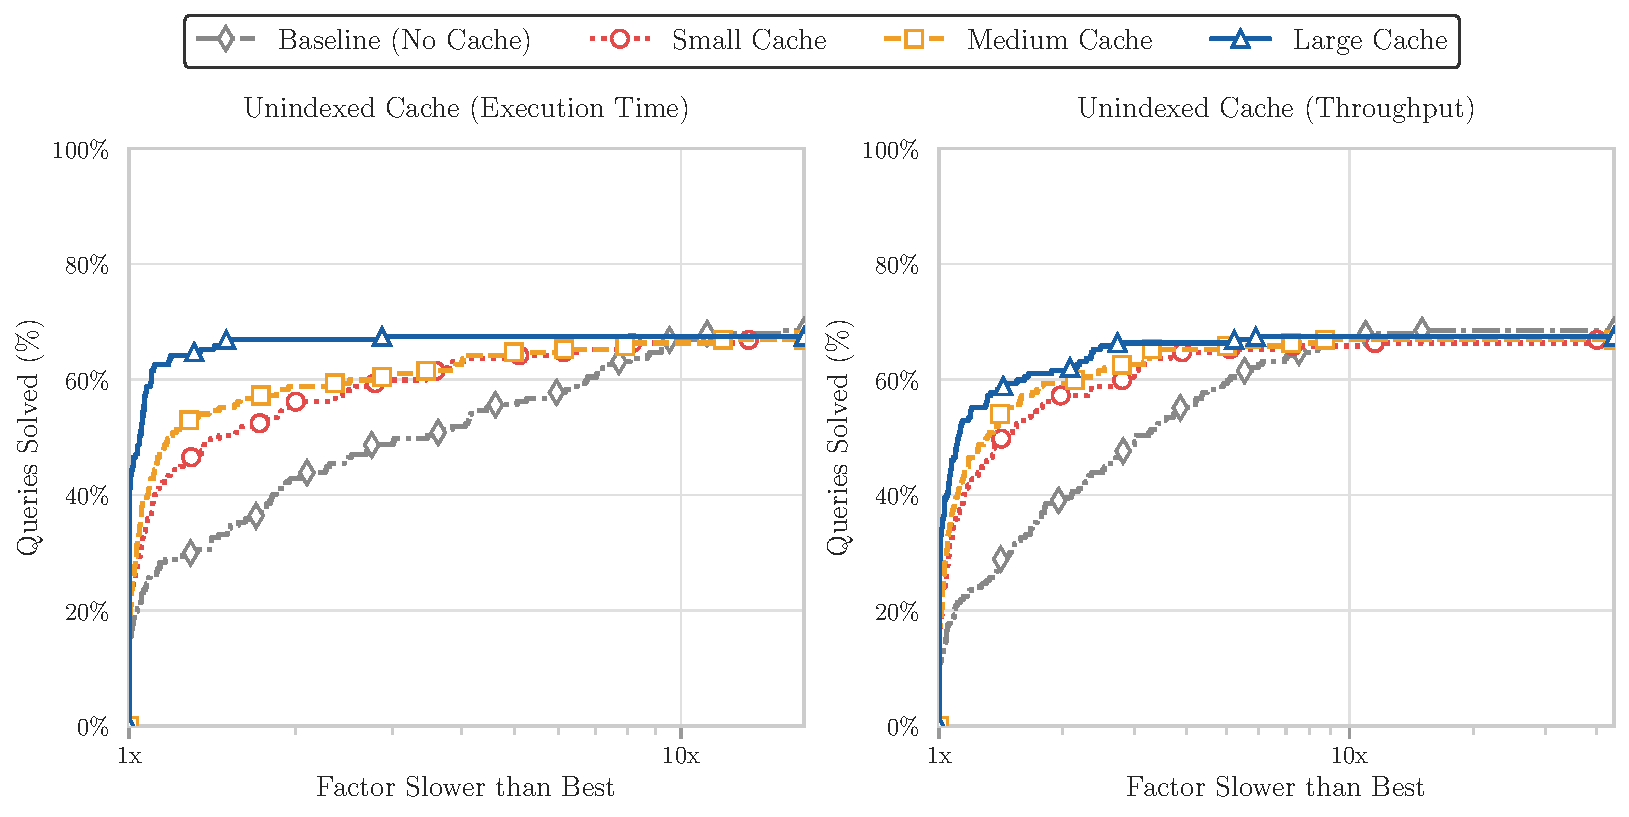
\includegraphics[width=\linewidth]{figures/performance_profile_normal_sequences_unindexed.pdf}
    \caption{Performance profiles of the LRU-based unindexed triples cache. 
    The y-axis shows the percentage of queries executing within a factor (x-axis) of the fastest algorithm. 
    Curves closer to the top-left indicate better overall performance. 
    The y-intercept ($x=1$) shows how often an algorithm is the outright fastest, 
    while the rightward trajectory demonstrates robustness 
    (e.g., $x=2, y=80\%$ means 80\% of queries execute within twice the fastest time).
    From the figure, we observe that all caching-based approaches outperform the no-cache baseline.}
    \label{fig:unindexed-lru-cache-performance}
\end{figure*}

\paragraph{Indexed LRU Cache}
As shown in Figure~\ref{fig:indexed-lru-cache-performance}, 
pre-indexing triples in the LRU cache accelerates successful query execution
but introduces higher initial overhead. 
When high cache eviction rates outweigh the efficiency gains of indexing, 
this ingestion cost slows down execution or causes timeouts. 
The figure illustrates this overhead, as the no-cache baseline ultimately solves a higher percentage 
of queries than the standard indexed cache as the line reaches a higher y-value. 

However, integrating cardinality estimation overcomes this limitation 
by enabling the query engine to generate more accurate query plans, 
increasing the percentage of solved queries and lowering execution times. 
Comparing the two estimation approaches, reachability-aware estimation 
outperforms reachability-agnostic estimation by ignoring irrelevant data. 
This effect is most pronounced in larger caches, where reachability-agnostic estimation 
yields only minor performance benefits, while reachability-aware estimation shows substantial improvements. 
This aligns with expectations: larger caches accumulate more irrelevant, 
out-of-context data, which the reachability-aware estimator successfully filters out.

\begin{figure*}[t]
    \centering
    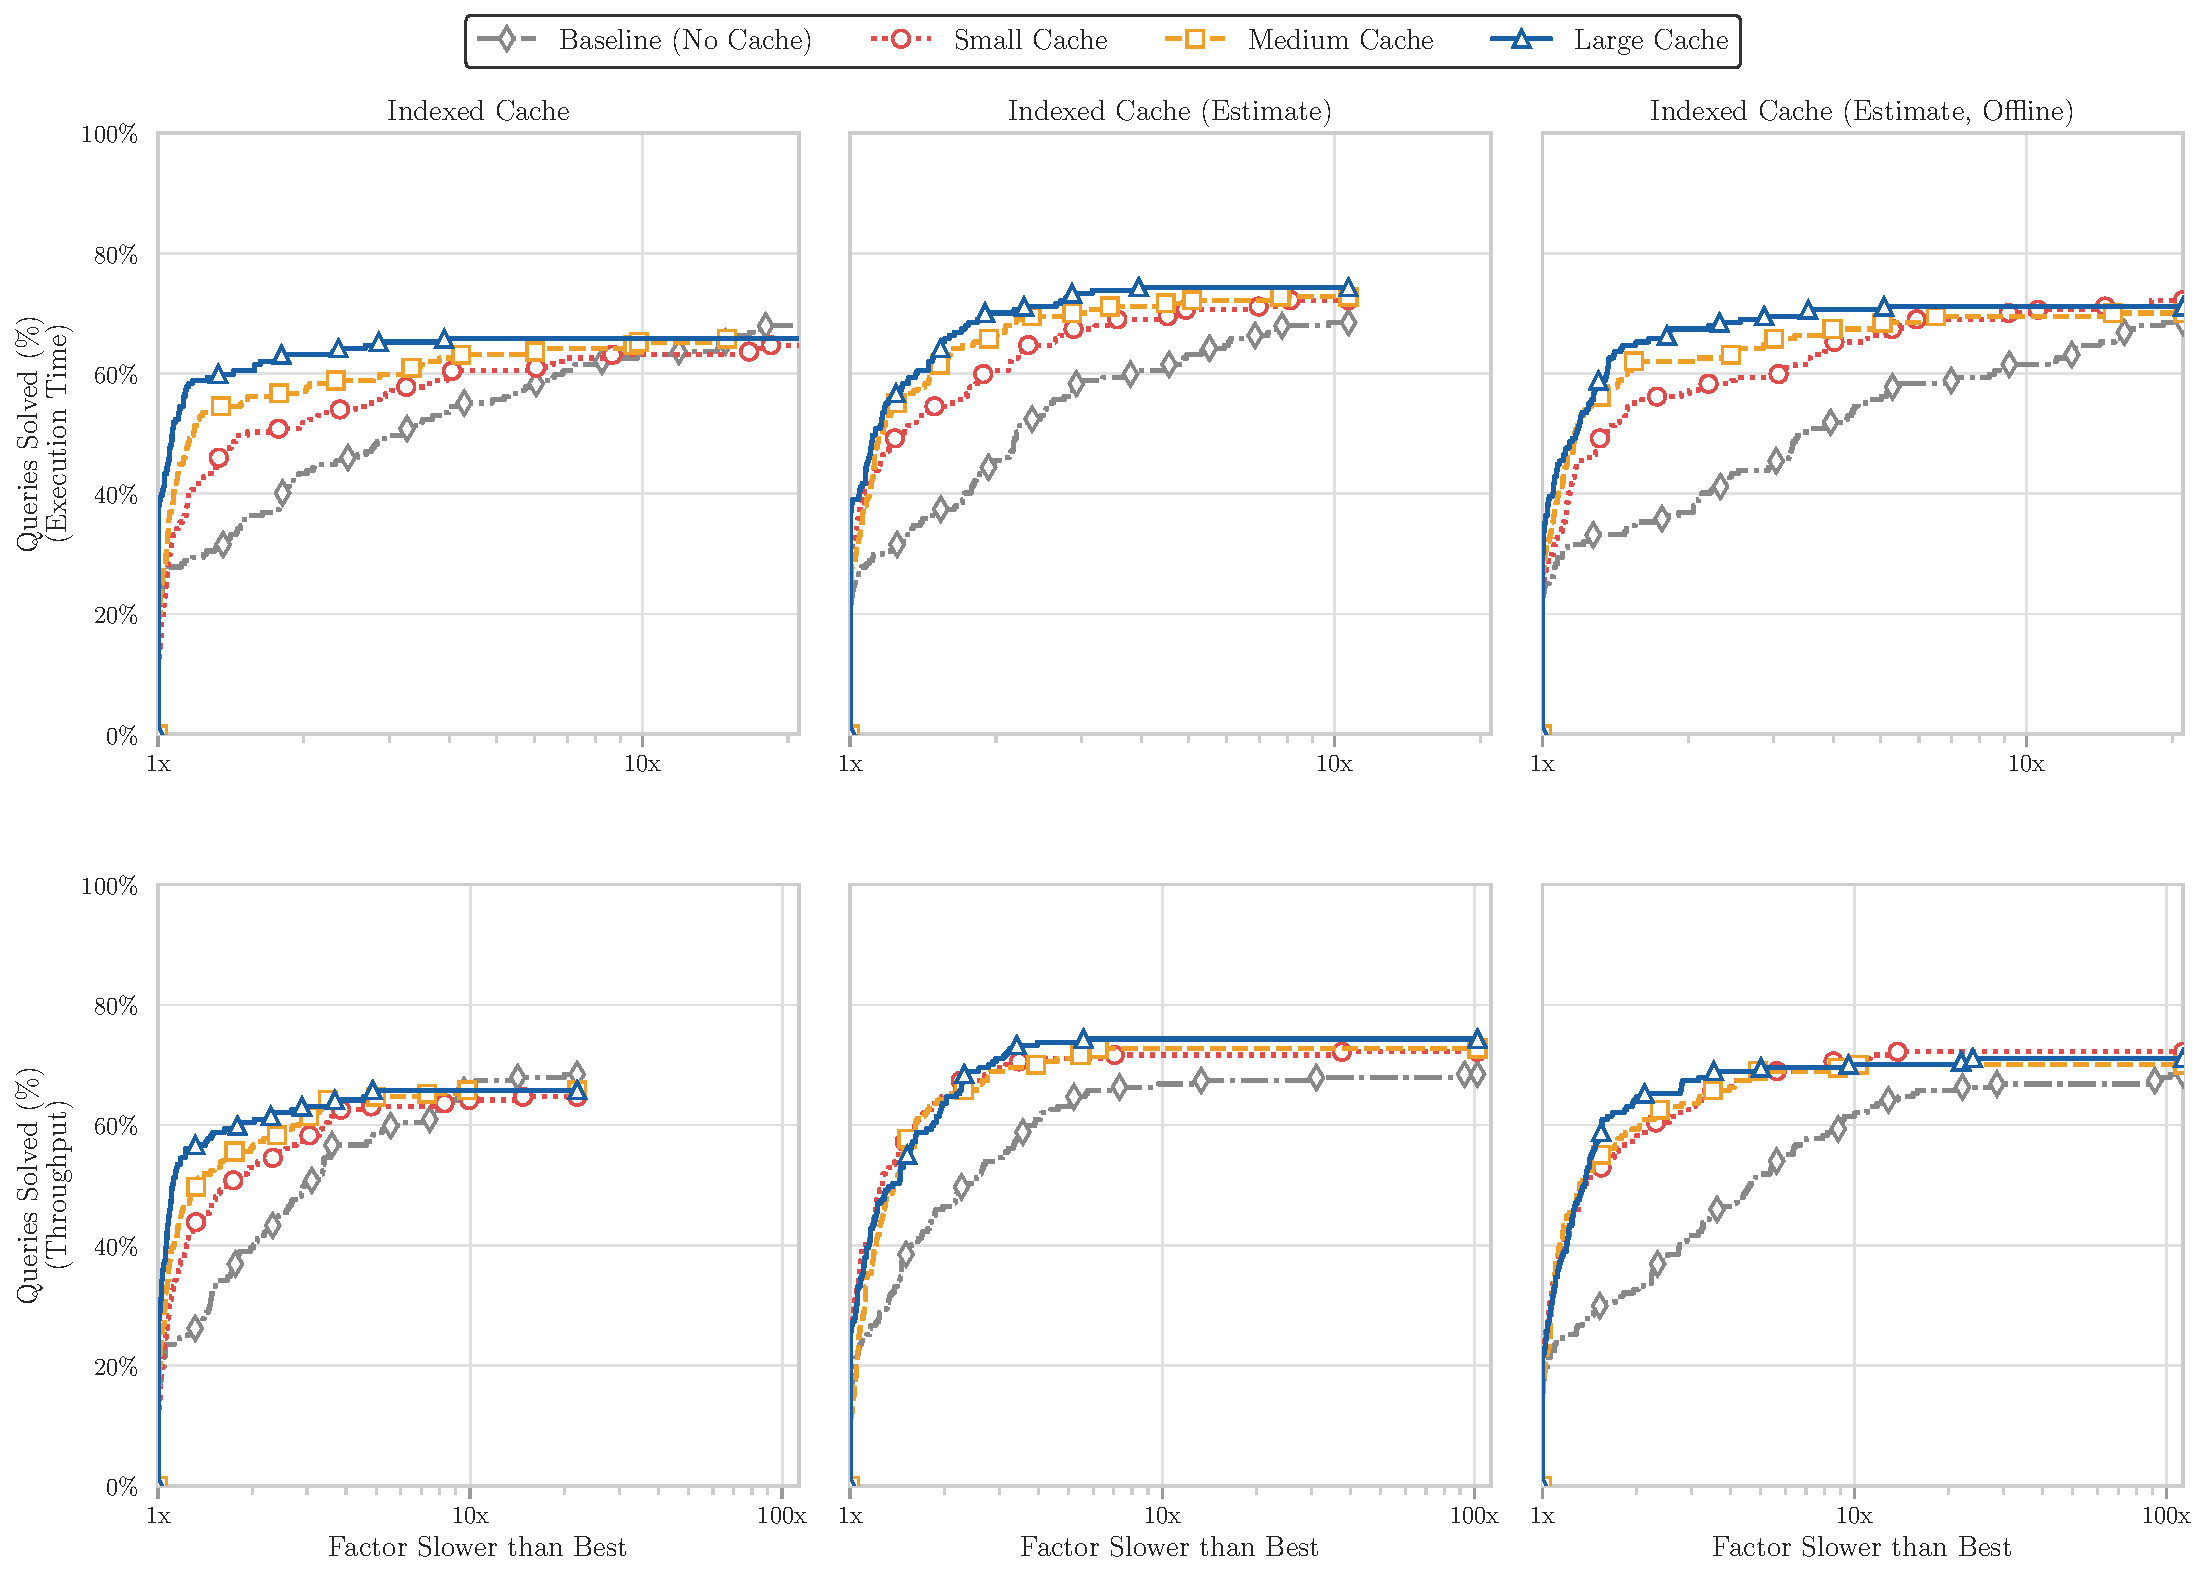
\includegraphics[width=\linewidth]{figures/performance_profile_normal_sequences_cache.pdf}
    \caption{Performance profiles of the LRU-based indexed cache family of algorithms. 
    The y-axis shows the percentage of queries executing within a factor (x-axis) of the fastest algorithm.}
    \label{fig:indexed-lru-cache-performance}
\end{figure*}


\paragraph{Memory-based Quad store Cache}
As shown in Figure~\ref{fig:quad-store-cache-performance}, 
the memory-based quad store cache exhibits high performance variance depending on the estimation strategy.
Without estimation (\textit{Indexed Store}), performance scales normally with capacity: 
the large cache achieves the best performance, while the medium and small caches sit lower 
but still reliably outperform the baseline. 
Similar to the LRU-based indexed cache, the baseline solves slightly more queries, indicating that the
performance overhead can cause query failures.
However, introducing online cardinality estimation (\textit{Indexed Store (Estimate)}) 
completely inverts the performance scaling observed without estimation, 
with the small and medium caches outperforming the large cache. 

The scaling nature of the performance penalty of cache size in estimation indicates that
executing count queries scales unfavorably as the cached quad store size increases.
Compared to the LRU-cache, which executes count triple pattern queries over small sources,
the quad store-based approach uses triple pattern queries over the entire quad store, but with
the graph term filled in to represent the current document.
For reachability-aware estimation the performance hit is not as big, especially in the
total execution time case.

\begin{figure*}[t]
    \centering
    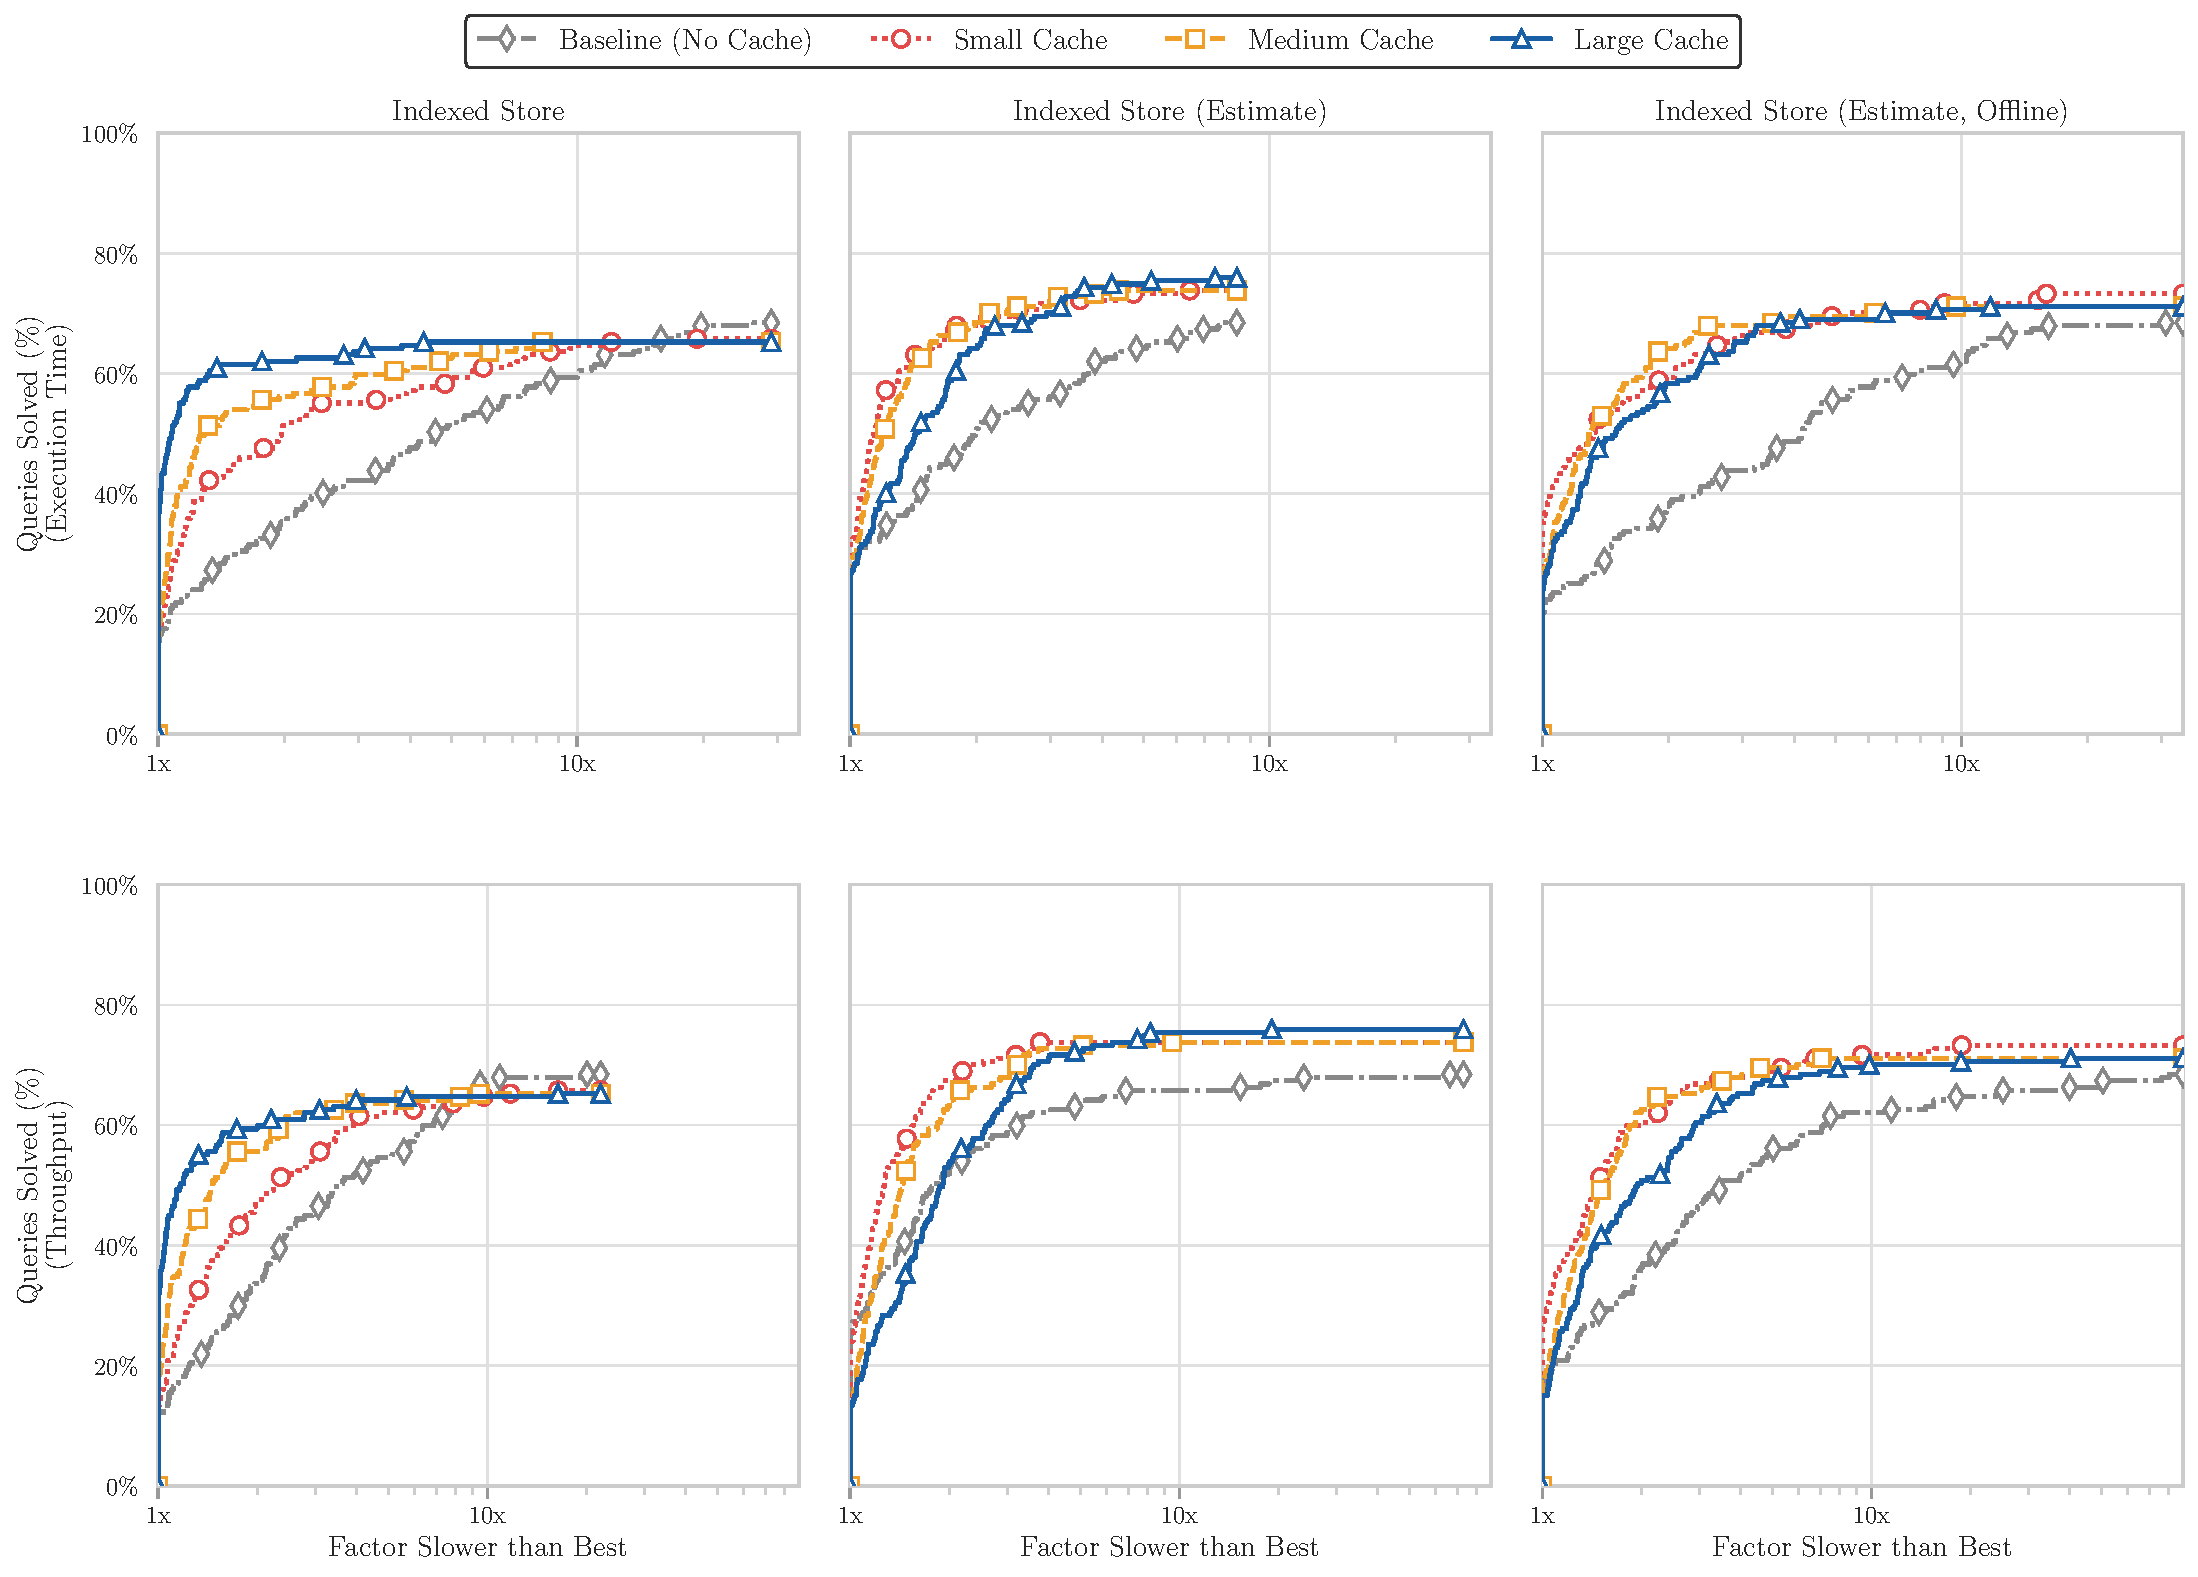
\includegraphics[width=\linewidth]{figures/performance_profile_normal_sequences_store.pdf}
    \caption{Performance profiles of the in-memory quad store cache family of algorithms. 
    The y-axis shows the percentage of queries executing within a factor (x-axis) of the fastest algorithm.}
    \label{fig:quad-store-cache-performance}
\end{figure*}

\paragraph{Disk-based Quad store Cache}

In Figure~\ref{fig:disk-store-cache-performance}, we see that the disk-based quad store cache performs....
\todo{PLACEHOLDER FIGURE}
\begin{figure*}[t]
    \centering
    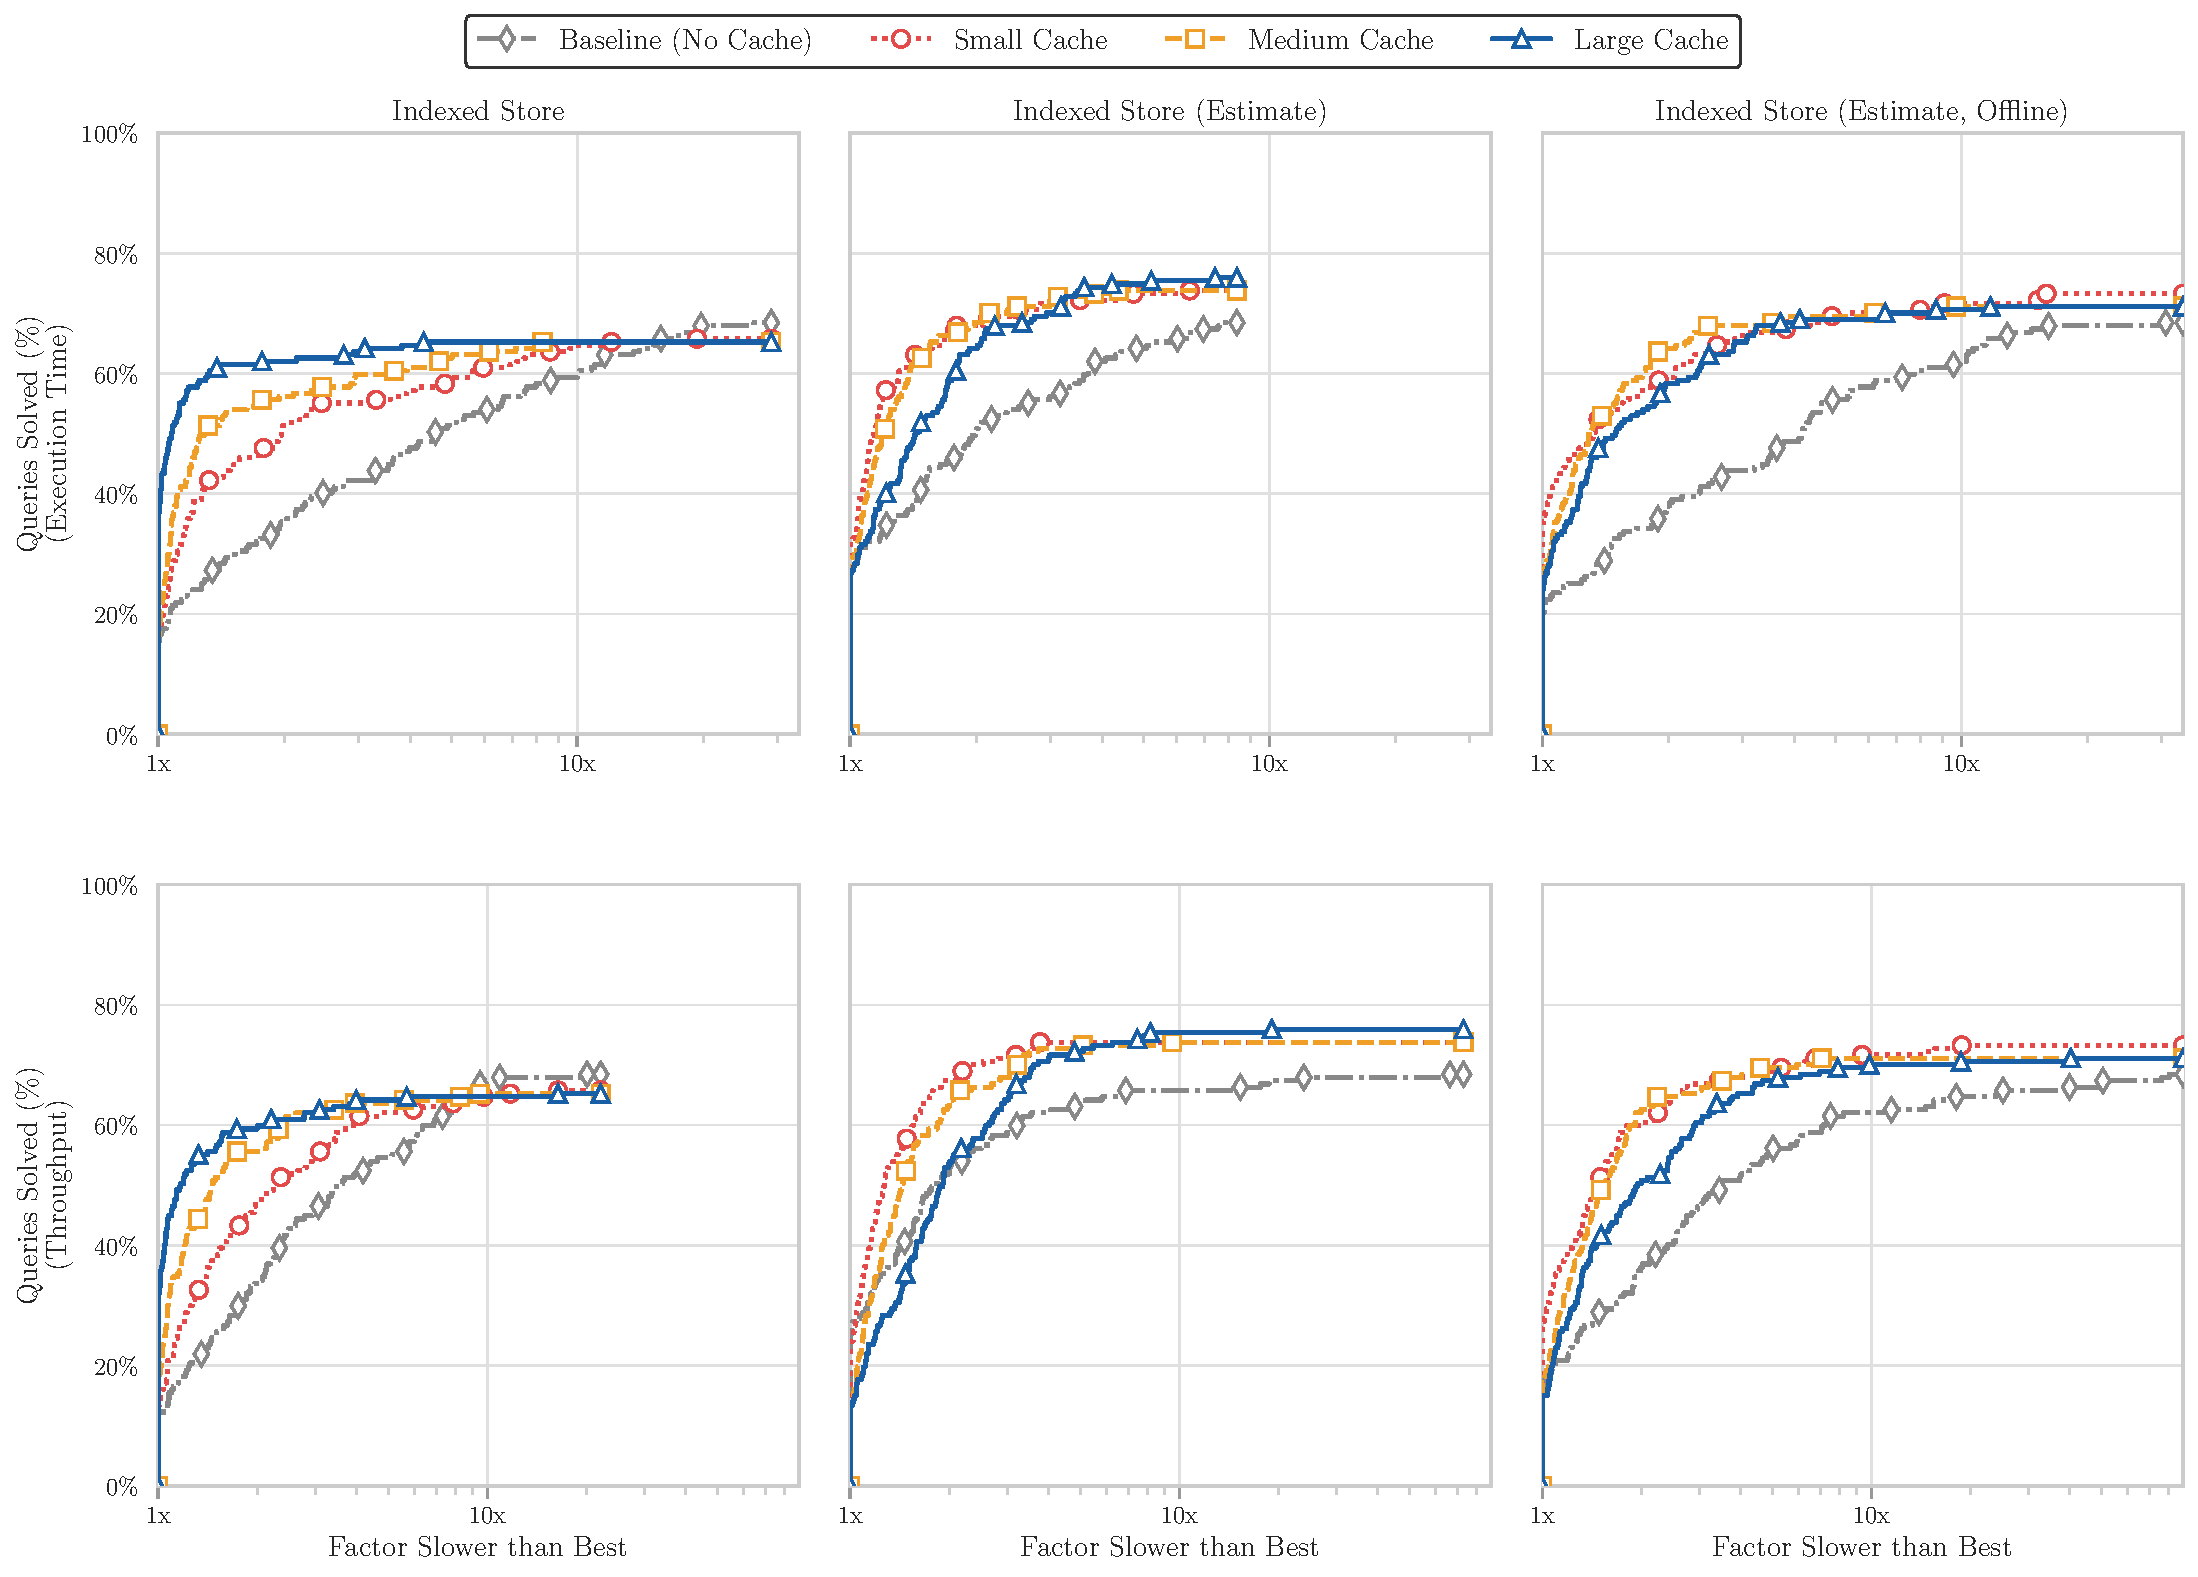
\includegraphics[width=\linewidth]{figures/performance_profile_normal_sequences_store.pdf}
    \caption{Performance profiles of the disk-based quad store cache family of algorithms. 
    The y-axis shows the percentage of queries executing within a factor (x-axis) of the fastest algorithm.
    \todo{PLACEHOLDER FIGURE}}
    \label{fig:disk-store-cache-performance}
\end{figure*}


\paragraph{Comparison Between Caching Algorithms}
\todo{Small section comparing the different caching algorithms and their performance characteristics.
for example how unindex cache mainly improves total execution time, how quad store seems best when
using small caches and LRU-cache scales better for bigger caches.}

\subsubsection{Cache Hitrates}
\todo{Optional section with hitrates and eviction percentages per cache size and algorithm.}


\subsection{Logical Session \& Interest Modeling Cache Performance}

Present a table showing the effect of logical sessions on cache performance. 
Include a metric for the delta number of unique data sources accessed 
during session switches to quantify data locality. 
Discuss the implications of these session dynamics for cache sizing 
and eviction policies.

\subsection{Refinement Patterns}

\todo{Write introduction to this section}

\subsubsection{Effect of chokepoints on query sequences}
\todo{This has a lot of repetition yes?}
We isolated the structural impact of individual query chokepoints through a controlled experiment comprising 80 single-query sequences.
Each sequence begins with a base query and sequentially applies a chain of two to five refinement patterns
from the benchmark's default refinement pattern set.
We repeated each sequence execution 10 times across the three distinct cache capacities (Small, Medium, and Large), 
and measure the cache hit rate, the number of unique data sources accessed, and the total execution time.
For this experiment we only use the LRU-based indexed cache, as we want to analyse the chokepoints 
and their effect on the cache in the simplest configuration.
To quantify the specific performance impact of each chokepoint, 
we mapped the refinement patterns to their underlying chokepoints 
and evaluated them using a linear mixed-effects regression model. 
The model predicts the performance delta ($\Delta Y$) between the current and previous query step. 
We categorize chokepoint operations into two classes: additions (denoted by an `a' suffix) 
and removals (denoted by an `r' suffix). 
A removal operation only occurs when the sequence reverts a previously applied refinement pattern, 
thereby dropping the associated chokepoint from the query. 
The chokepoints added in a given refinement step are represented as a binary vector $X_{t}$, 
where each element indicates the presence (1) or absence (0) of a specific chokepoint. 
These vectors are then used as predictors in the regression model, 
in combination with the previous query's performance metrics ($Y_{t-1}$) to account for the baseline state of the system.
The full regression model is expressed as follows:
\begin{equation}
    \Delta Y_{i,t} = \gamma Y_{i,t-1} + \mathbf{T}_{i,t}^{\top} \boldsymbol{\beta} + u_i + \epsilon_{i,t},
\end{equation}
where $\Delta Y_{i,t}$ is the performance delta for sequence $i$ at refinement step $t$,
$Y_{i,t-1}$ is the previous steps independent variable value, 
$\mathbf{T}_{i,t}$ is a binary indicator vector of the applied chokepoints, 
$\boldsymbol{\beta}$ is the vector of fixed effects estimating the isolated impact of each pattern,
$u_i$ is a sequence-specific random intercept absorbing unobserved heterogeneity across base queries,
and $\epsilon_{i,t}$ is the standard residual error.


Figure~\ref{fig:chokepoint_regression_coefficients} shows the estimated effect of each chokepoint on performance. 
Full regression results are in Appendix~\ref{app:regression_tables} \todo{Verify appendix or supplemental material}.

We observe two types of chokepoint behavior. 
First, modifying some patterns hurts performance in both directions. 
For example, both adding and removing \texttt{T\_3} (increasing required traversal hops) reduces the hit rate and increases execution time.
This reveals a strong cache invalidation penalty: changing the refined query breaks the cache, overwriting much of it and evicting useful data.
From this, we can observe that caching requires a \textit{scan-resistant} algorithm.    

Second, patterns like \texttt{T\_2} (new instantiation values) and \texttt{P\_4} (non-selective triple patterns) have reversible effects. 
Adding these chokepoints drops performance, but removing them improves the hit rate and speeds up execution. 
In these cases, the cache is able to maintain useful data across the refinement, and the chokepoint itself is the primary cause of performance degradation.
Finally, across all patterns, chokepoints that increase the number of accessed data sources consistently lower the cache hit rate.

\paragraph{Implications for Refinement Pattern Design}
From our analysis, we find important weaknesses in our tested caching algorithms. 
We demonstrate that structural mutations like \texttt{T\_3} trigger severe cache invalidation penalties, heavily degrading performance. 
Conversely, the reversible nature of patterns like \texttt{T\_2} proves that caches can successfully maintain temporal locality 
even when the instantiation value, and thus the traversal starting point, changes. 
These findings highlight the importance of our refinement sequence generator and the mapping of refinement patterns to chokepoints.
This mapping allows us to isolate the structural impact of each chokepoint and thus analyse the strengths and weaknesses of a given caching algorithm.
Furthermore, because our sequence generation is dynamically configurable, 
it serves as a targeted diagnostic tool for future systems research. 
Developers can easily extend our default configurations to isolate specific chokepoints, 
allowing them to custom-build stress tests that target the unique operational challenges of their own caching architectures.


The resulting coefficients are given in Figure~\ref{fig:chokepoint_regression_coefficients}, 
where the x-axis represents the estimated effect size of each chokepoint on the performance delta, and the y-axis lists the chokepoints.
For full regression results, we refer to the \todo{Where to put them?}.
From the figure we find that for some chokepoints, such as T.3 (increasing the number of hops required to obtain the data), 
both addition and removal significantly reduce cache hit rate and increase execution time.
Indicating that the chokepoint causes the cache to evict previously cached data, which causes it to underperform when the chokepoint is removed.
Another type of chokepoint, is where the addition of the chokepoint reduces the hitrate and increases execution time, 
while removing it increases hitrate while reducing execution time, such as T.2 (new instantiation value) and P.4 (adding non-selective triple patterns).
Counterintuitively, for chokepoints such as `P.3.r', `P.2.r', and `P.1.a', the large cache has a smaller positive effect 
on hitrate compared to the smaller caches.
As cache hitrate is bound by 1.0, the large cache will have less room for improvement compared to smaller caches, which explains the smaller observed effect.
This is supported by the average hitrates over all queries, which are $0.51$, $0.61$, and $0.66$ for the small, medium, and large caches respectively and the
significant negative coefficient of the lagged cache hitrate value in the regression model, which indicates that a higher previous hitrate reduces the expected change in hitrate.

Finally, we find that in general, chokepoints that significantly increase the number of sources accessed, significantly reduce cache hit rate and vice versa.

\begin{figure*}[htpb]
    \centering
    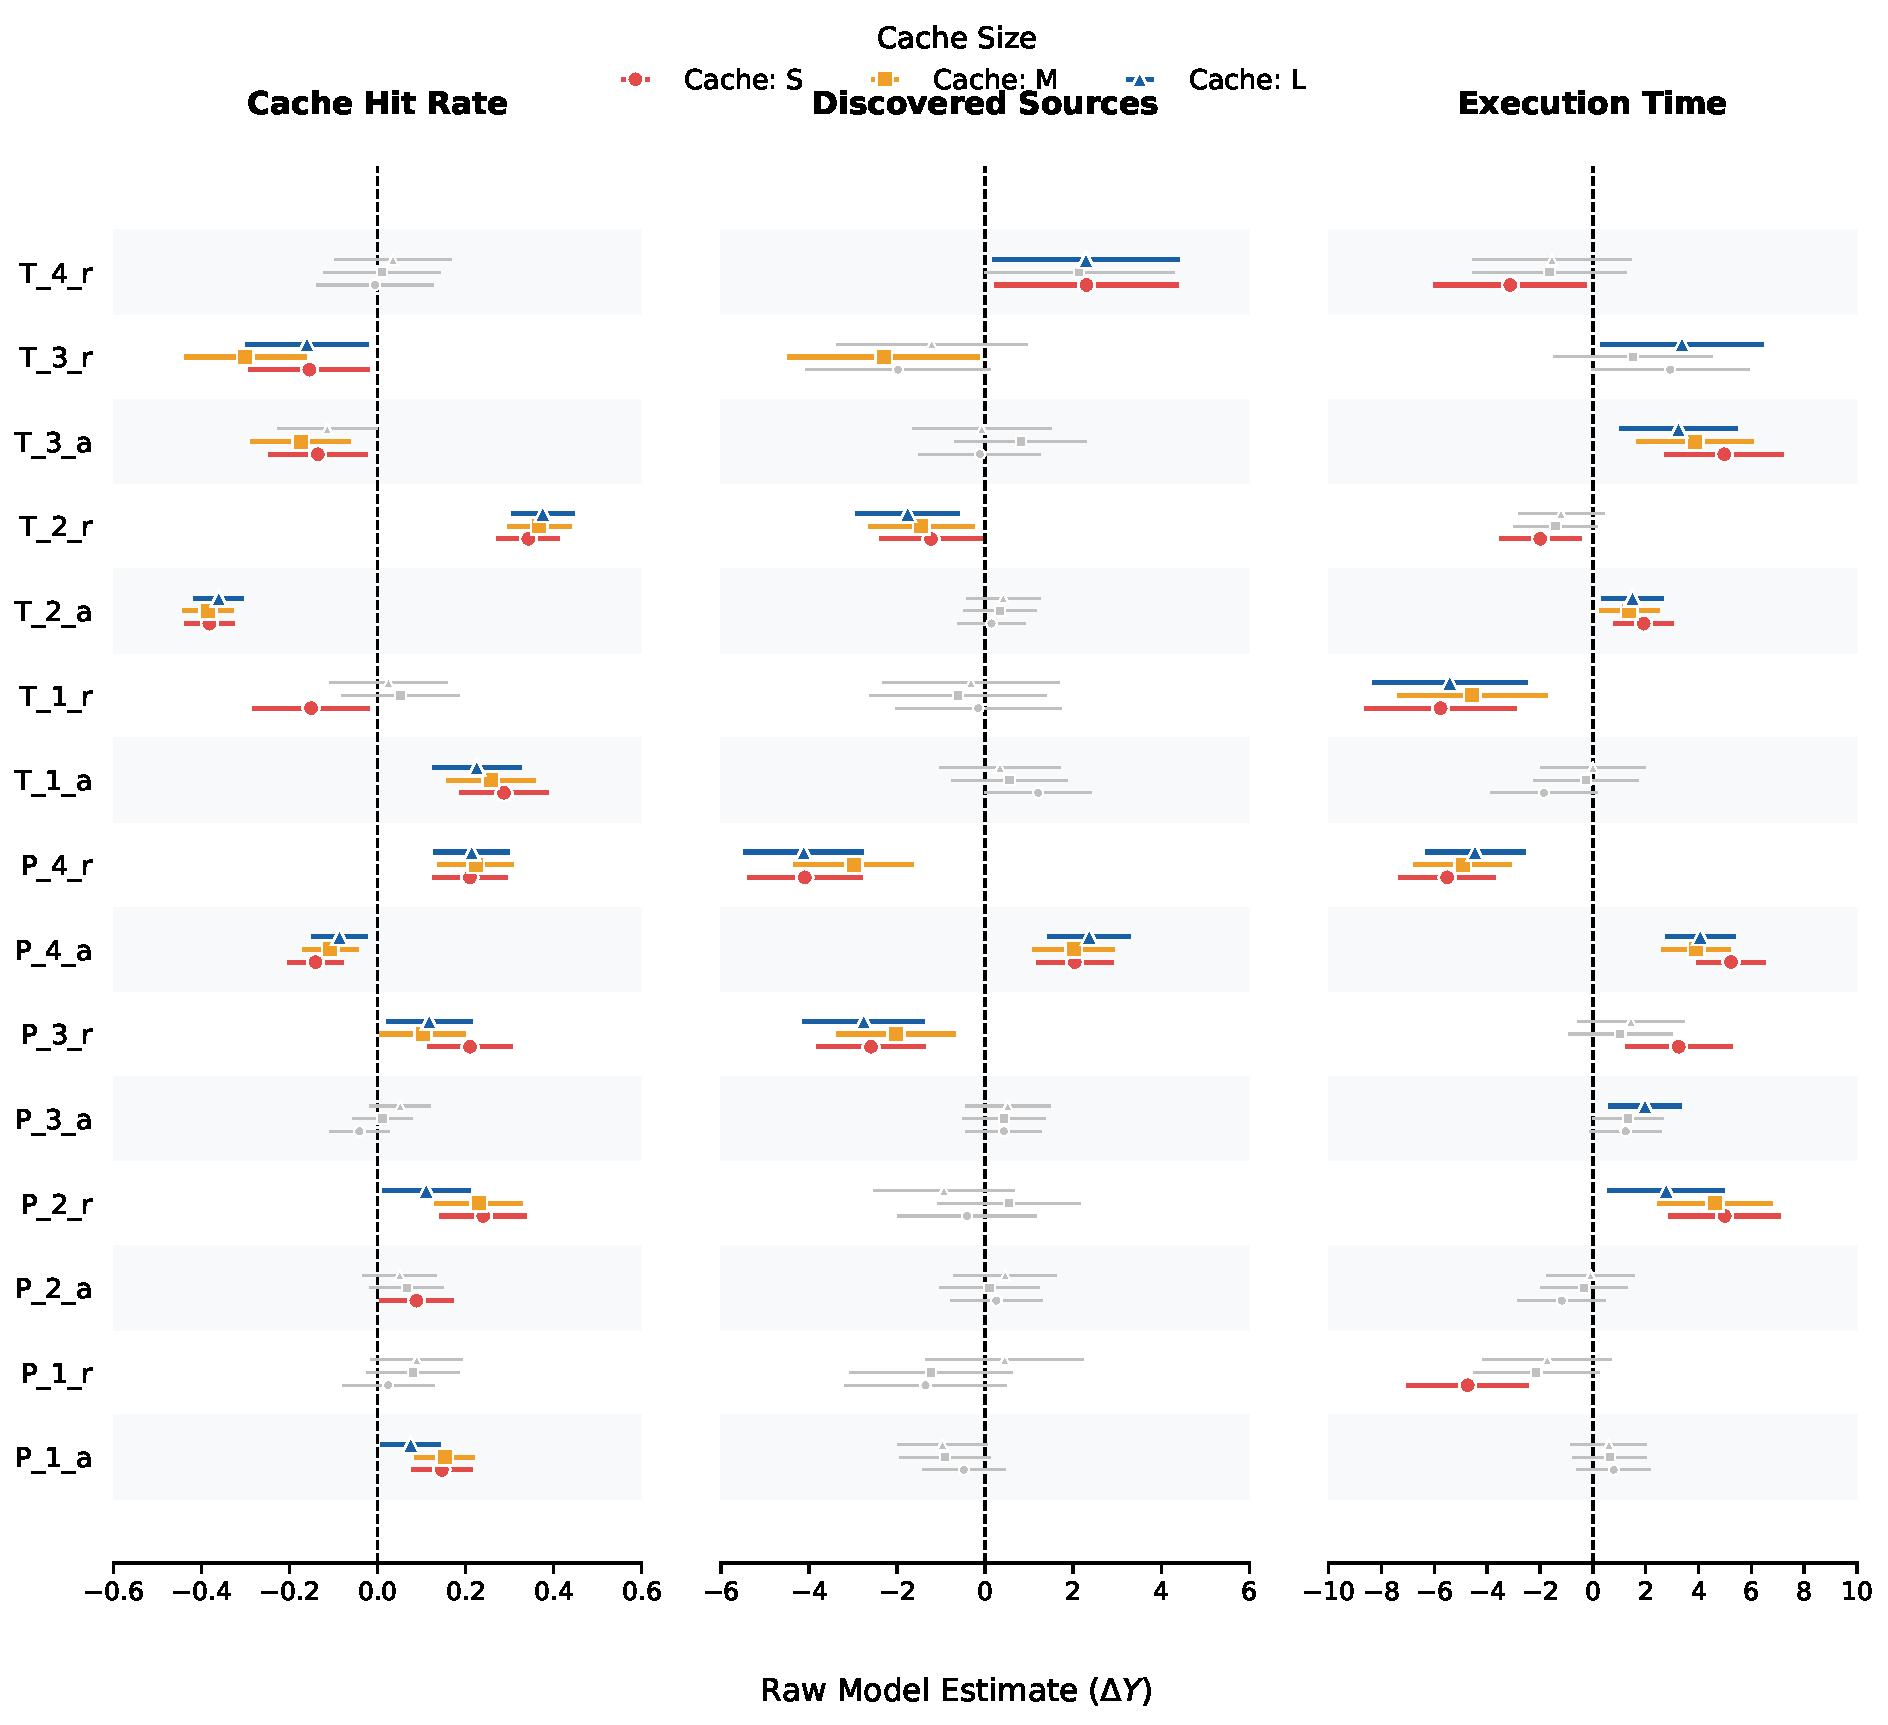
\includegraphics[width=\textwidth]{figures/faceted_forest_figure.pdf}
    \caption{Marginal fixed effects of refinement pattern additions (\texttt{-a}) and removals (\texttt{-r}) on query performance 
        across Small (S), Medium (M), and Large (L) cache capacities. 
        The plot reports the unstandardized absolute expected change ($\Delta Y$) for Cache Hit Rate, Discovered Sources, and Execution Time.
        For both discovered sources and execution time, the plot uses signed log-counts and signed log-milliseconds, respectively.
        Error bars represent $95\%$ confidence intervals and statistically insignificant estimates $(p \ge 0.05)$ are rendered in gray. 
        Undoing the traversal chokepoint changing the instantiation value of the query significantly improves cache hit rate (+.35) and
        reduces the number of unique data sources accessed. However, its effect on execution time is on the edge of significance.}
    \label{fig:chokepoint_regression_coefficients}
\end{figure*}

\subsubsection{Effect of Refinement Depth on Performance}
Next, using default query generation, assess the effect of refinement depth 
on cache performance, followed by implications for cache sizing 
and eviction policies.


\subsection{Comparison to Alternative Evaluation Methods}

The final step in our evaluation is to compare the performance outcomes obtained from our benchmark
against alternative evaluation methods from literature. \todo{Mention random / synthetic}


Compare SolidSessionBench's performance outcomes against alternative 
evaluation methods, specifically micro-benchmarks and random query sequences. 
Highlight differing performance characteristics, identify the analytical 
shortcomings of these alternative methods, explain how their resulting 
conclusions mislead, and demonstrate how this sequence-based benchmark 
resolves those issues.

\paragraph{Microbenchmarks-Theoretical Hit Rate Analysis}
Cache literature extensively uses microbenchmarks of various forms 
to analyze caching performance~\cite{nicholson2024hpcache,hartig2011caching}.
To compare the conclusions of such a benchmark to the conclusions of the benchmark introduced in this paper
we investigate theoretical caching speedup without management costs, 
by executing each query template twice with simulated cache miss probabilities. 
We excluded the estimation-based approaches,
as using the full cache for estimation would skew the results for miss rates above zero.

Figure~\ref{fig:theoretical_cache_performance} shows representative performance profiles for the workload. 
Most templates (8 out of 12) show reliable improvement that scales with the hit rate for both algorithms. 
However, certain long-running queries (e.g., interactive-discover-6, 7, and short-3) show no speedup, 
and some even experience slowdowns. 
These templates traverse many solid pods but do not require all traversed data. 
We hypothesize that rapidly serving documents from an in-memory cache overwhelms the system with data, 
slowing result production. 
Conversely, HTTP network latency gives the JavaScript event loop time to process the join execution pipeline, 
yielding initial results faster since only the first few requests are needed.

In general, using an indexed cache (store-based or LRU) improves performance more than an unindexed cache,
however, this also comes with higher cache management costs, which are not accounted for when using theoretical hit rates.
\todo{See about disk-base caching}
\todo{Circle back to our general evaluation to see how the conclusions differ}

\begin{figure*}[!h]
    \centering
    % Ensure the filename matches your generated PDF
    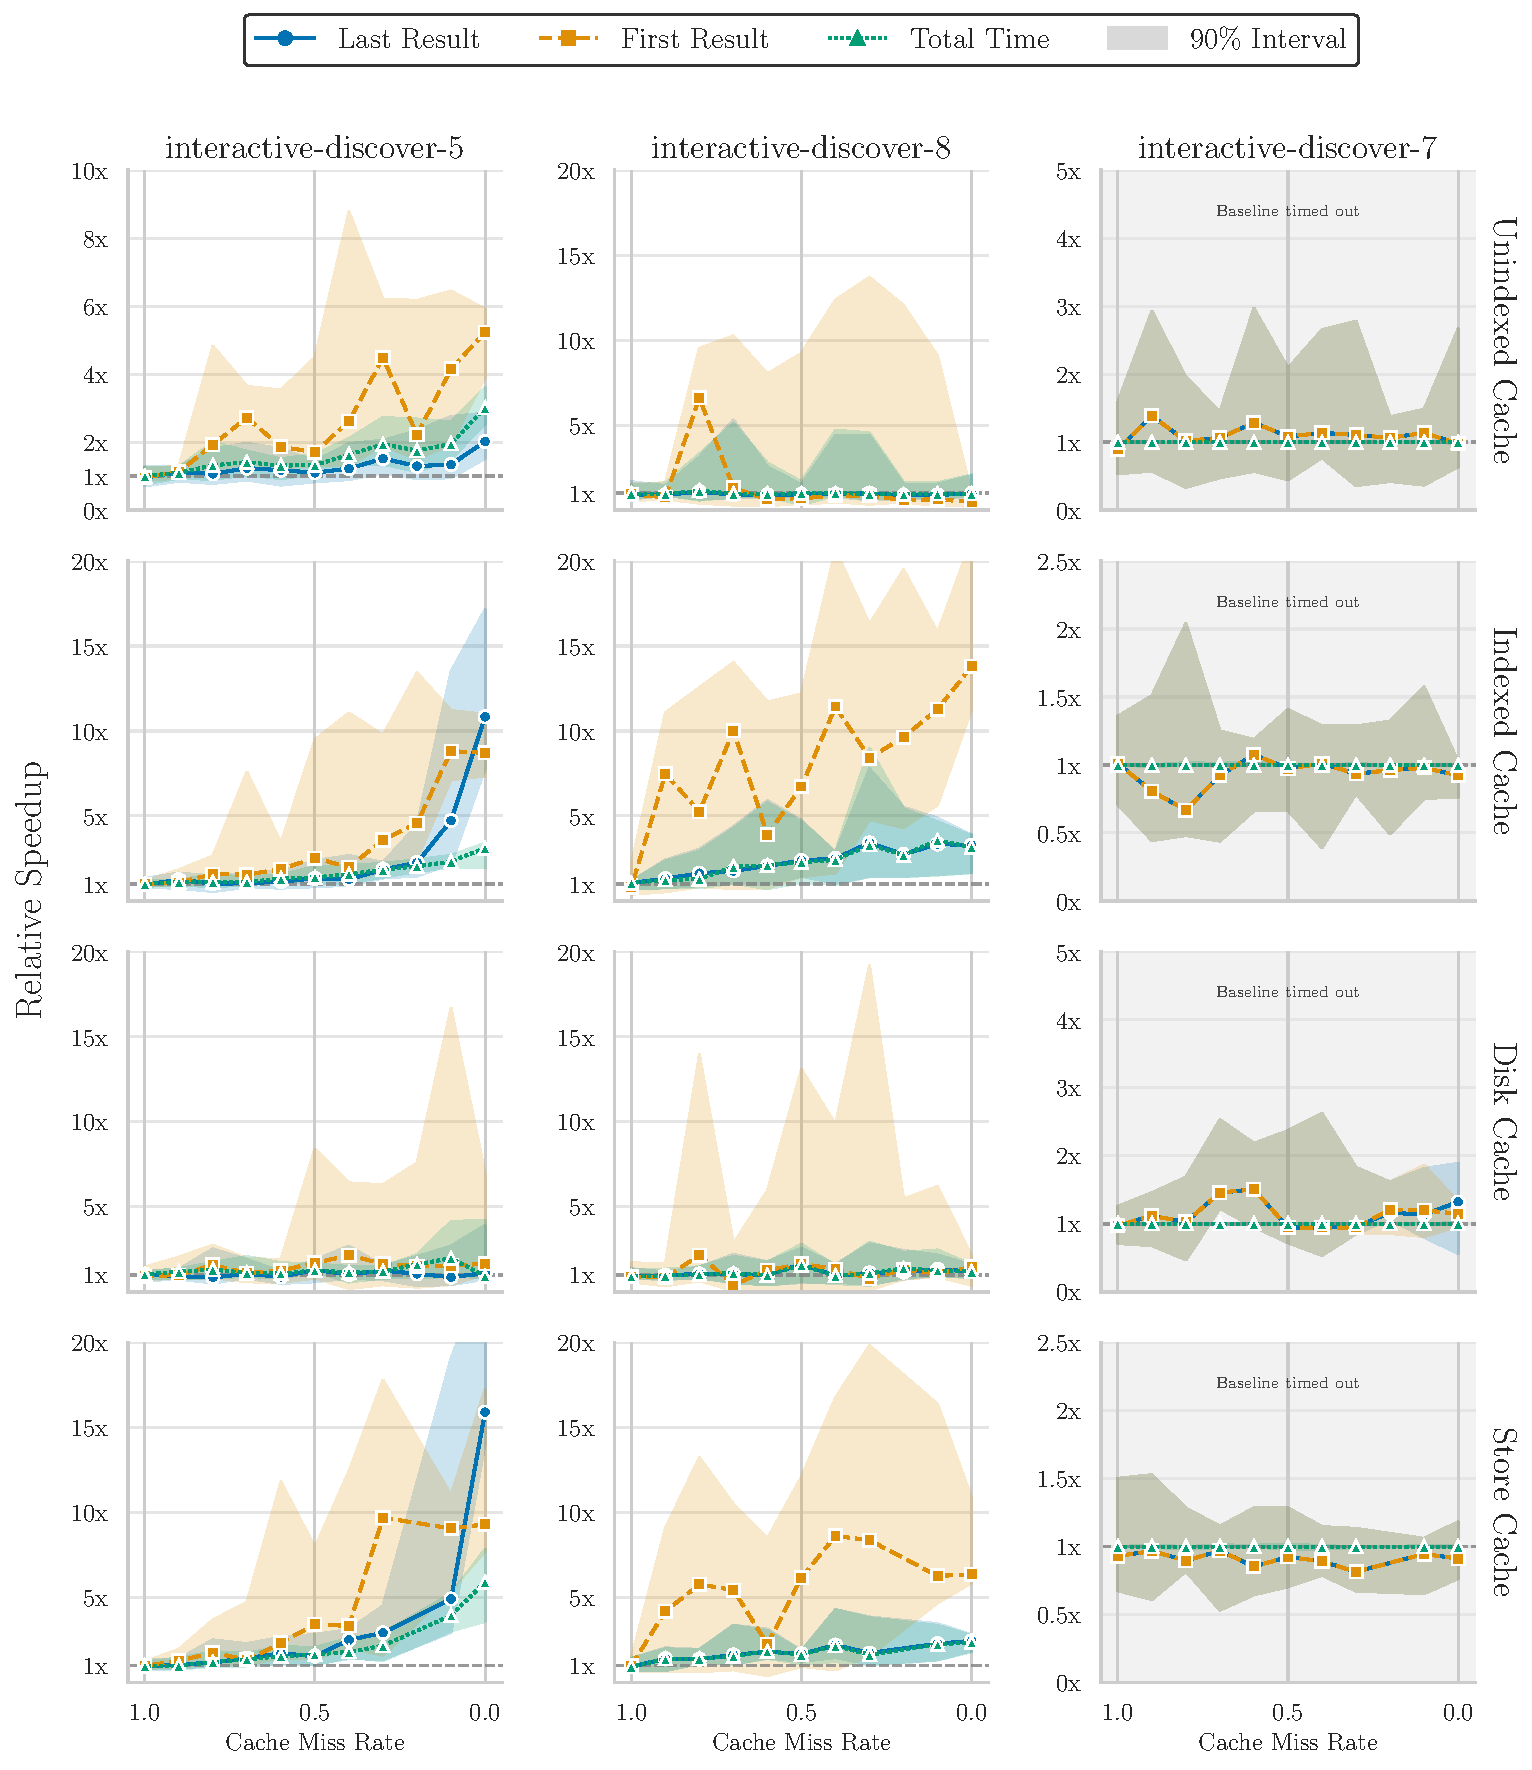
\includegraphics[width=\textwidth]{figures/synth_hit_rate_reduced_combined.pdf}
    \caption{ Performance of unindexed, LRU indexed, In-memory store, and Disk-based store caches 
    across representative query templates. The y-axis shows the mean speedup relative 
    to a baseline with a 0\% hit rate. Shaded regions denote the 90th percentile
    \todo{Placeholder disk figure}}
    \label{fig:theoretical_cache_performance}
\end{figure*}

\paragraph{Random Query Sequences}



\paragraph{Scope and Limitations}
We evaluate SolidSessionBench against microbenchmarks and random sequences, 
but explicitly exclude hand-crafted scenarios and simple distributions.
Hand-crafted methods lack scalability, while simple distributions fail to capture complex user habits.
By automating logical sessions and user interests, our benchmark functions as a scalable superset of both approaches,
making direct comparison redundant. 
By contrast, the compared methods do not incorporate these sequence attributes, 
and our results show this omission risks drawing inaccurate conclusions.

% We evaluate our benchmark using a scale 0.1 SolidBench dataset comprising 158,233 RDF files,
% 1,531 vaults, and 3,556,159 triples. 
% Applying the default hyperparameters from Table~\ref{tab:generation_hyperparameters},
% we generated 8 sequences totaling 192 interactive-workload queries, encompassing both discover and short templates.
% Experiments were conducted on an Ubuntu 20.04 machine (Intel Core i5-9400) with 16 GB RAM and a 180-second timeout.
% To minimize variance and simulate realistic networks, we repeated each sequence 10 times with 70–90 ms injected latency 
% to simulate realistic network conditions.
% Caches were scoped to individual sequences, ensuring no state was shared between repetitions. 

% These experiments aim to test our sequence generation by assessing how our design choices influence 
% query correlation, measured via cache hit rates and evictions, 
% and to establish a caching performance baseline for a Link Traversal-based Query Processing (LTQP) engine.
% While we report speedups to demonstrate utility, the primary focus is benchmark validation rather than exhaustive algorithm evaluation.  


% We evaluate our benchmark using a scale 0.1 SolidBench dataset 
% (158,233 RDF files, 1,531 vaults, 3,556,159 triples). 
% Using the default hyperparameters in Table~\ref{tab:generation_hyperparameters}, 
% we generate 8 sequences totaling 192 queries. 
% These queries are from the interactive workload, are split into discover and short queries,
% with multiple templates belonging to either of these groups.
% Experiments run on an Ubuntu 20.04 machine (Intel Core i5-9400) 
% with 16 GB RAM allocated to the engine and a 180-second query timeout. 
% We repeat each sequence 10 times to minimize variance and 
% inject a uniform 70–90 ms latency to simulate a realistic network environment.
% The cache is scoped for a sequence, meaning no cache-state is shared between different executions or repetitions of
% sequences.

% These experiments serve two goals. 
% Primarily, we validate the sequence generation by assessing how our three 
% design choices impact query correlation, measured via cache \textit{hit rates} and \textit{evictions}. 
% Secondarily, we establish a caching performance baseline for a LTQP engine. 
% While we report execution speedups to demonstrate the benchmark's utility, 
% our focus is on validating the benchmark design rather than exhaustively evaluating the caching algorithms.

% \rt{Can you briefly hint to the subsections that will come hereafter? (so the reader knows what to expect)}

% \subsection{Global Cache Performance}

% Figure~\ref{fig:global_cache_performance} compares performance profiles~\cite{dolan2002benchmarking} 
% for each approach against the no-cache baseline. 
% As expected, all caching methods outperform the baseline.

% \begin{figure*}[t]
%     \centering
%     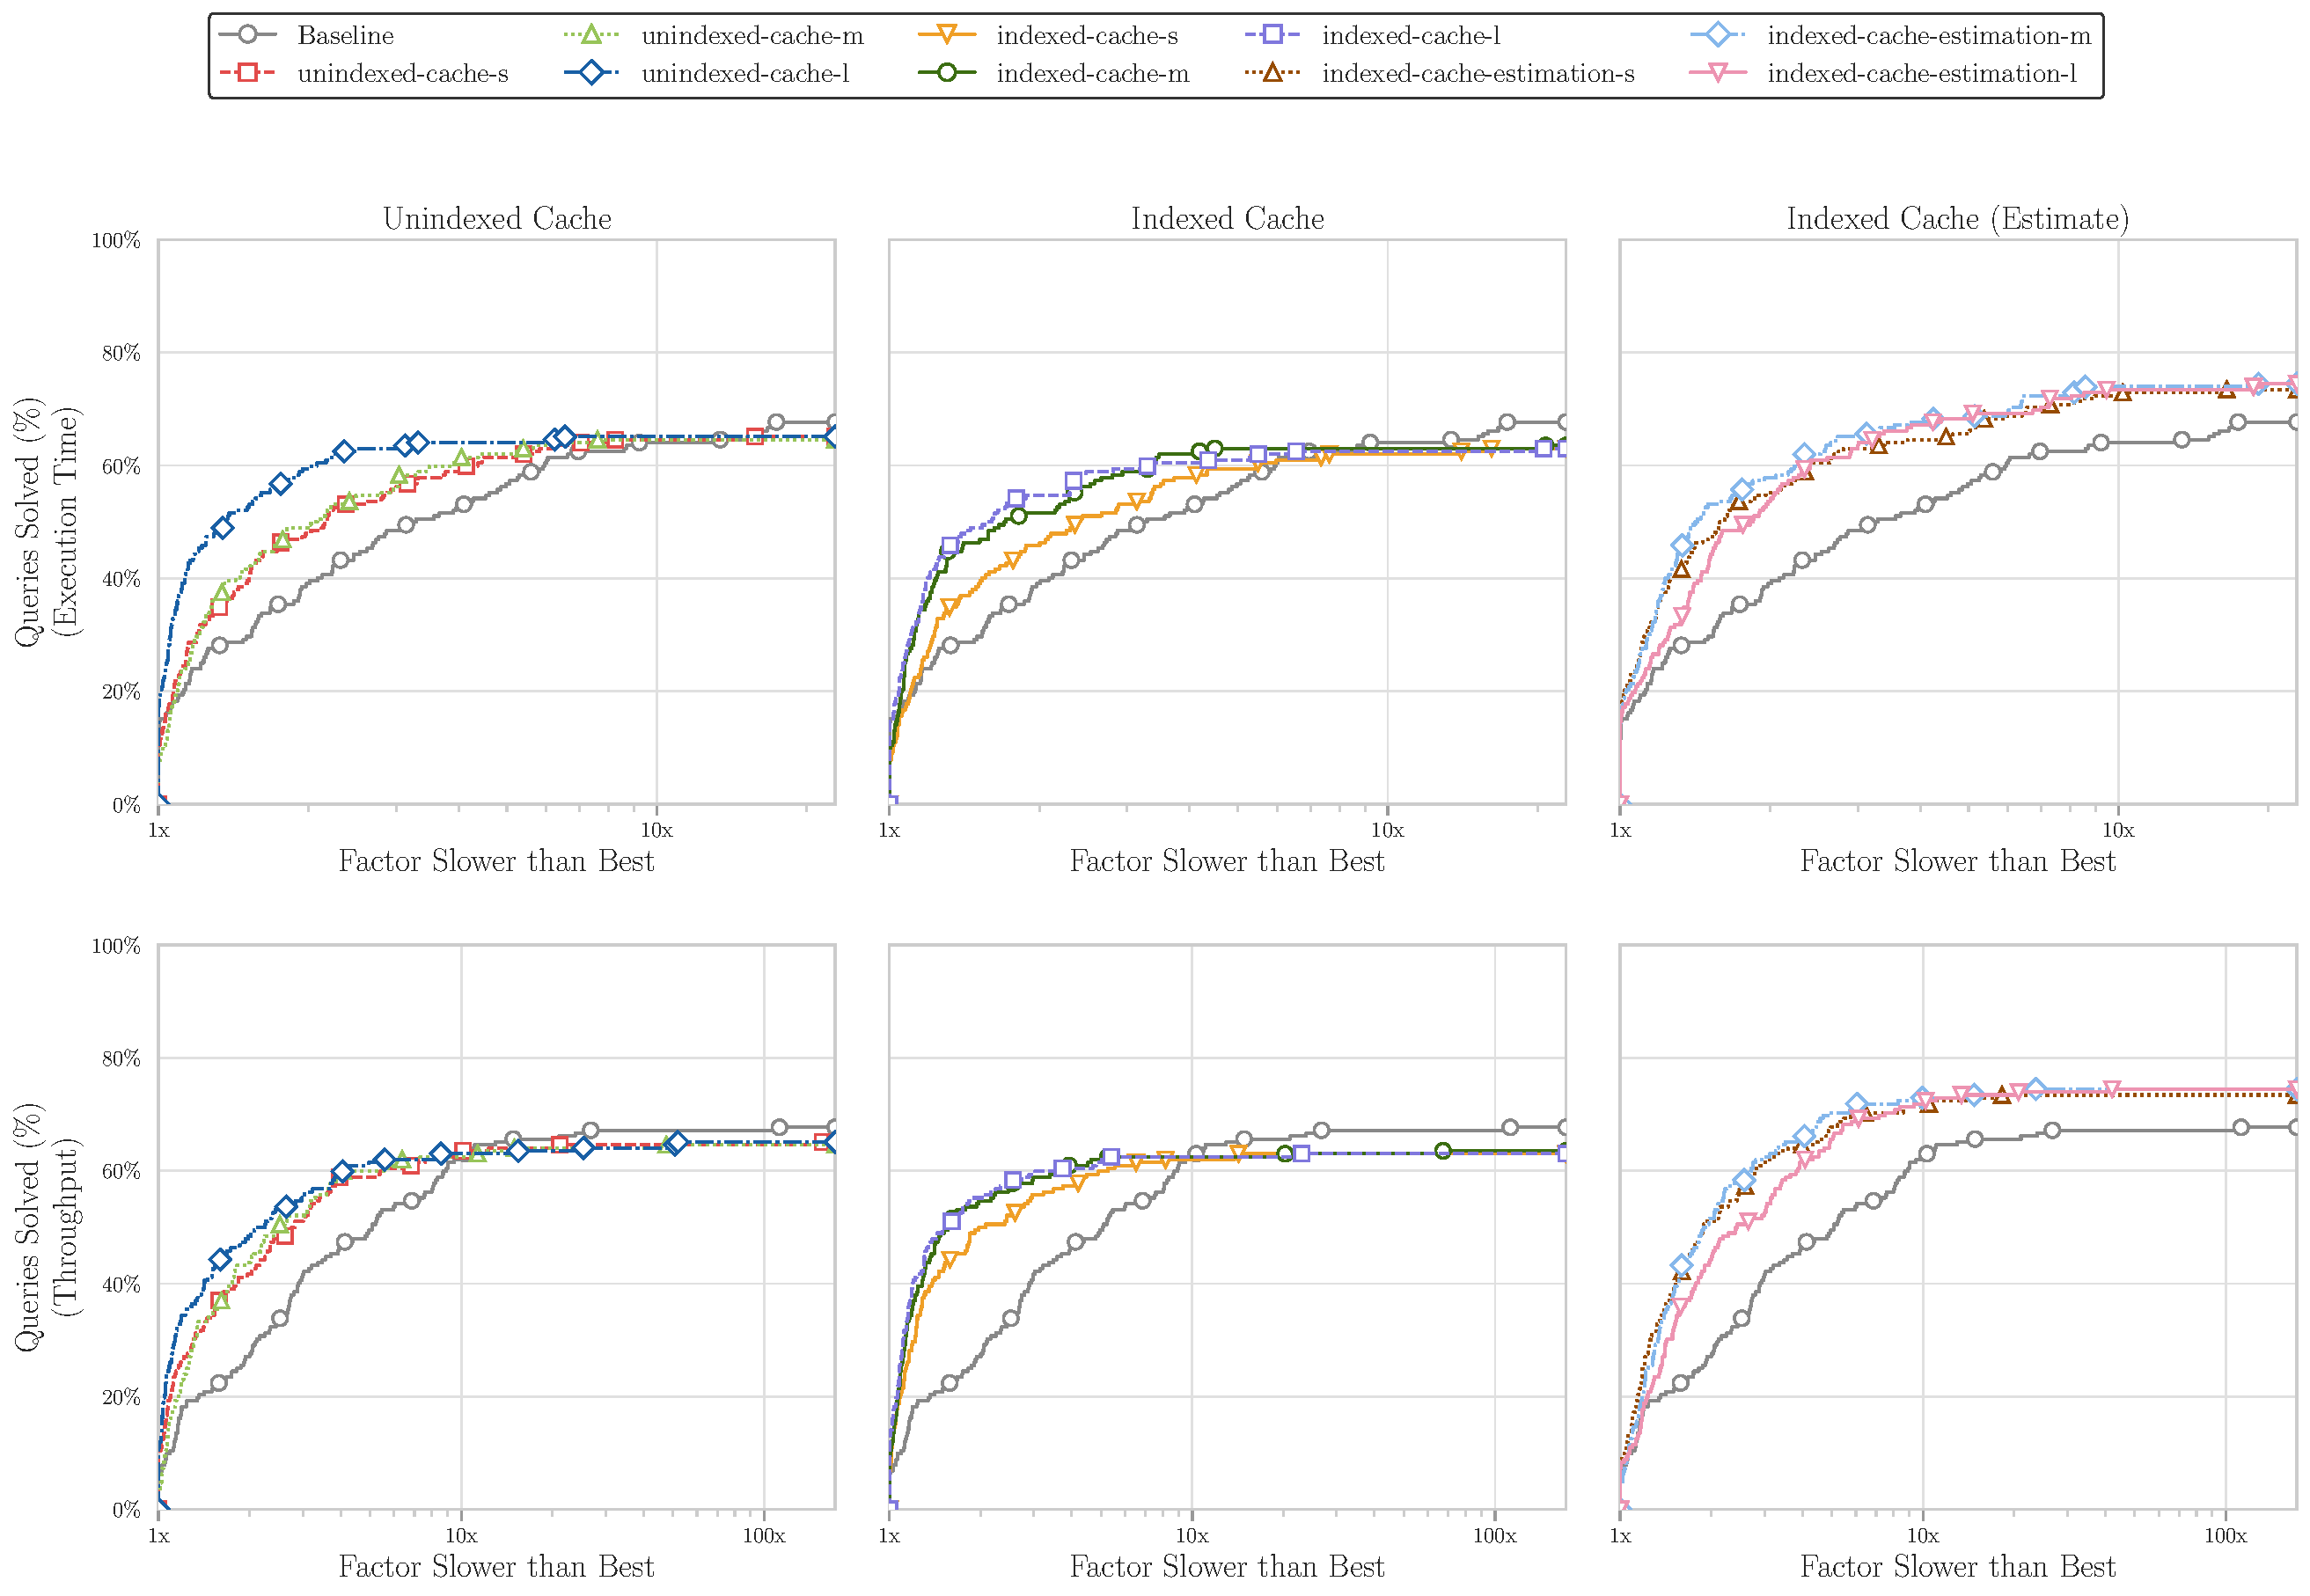
\includegraphics[width=\linewidth]{figures/performance_profile.pdf}
%     \caption{Performance profiles of the tested cache algorithms. 
%     The y-axis shows the percentage of queries executing within a factor (x-axis) of the fastest algorithm. 
%     Curves closer to the top-left indicate better overall performance. 
%     The y-intercept ($x=1$) shows how often an algorithm is the outright fastest, 
%     while the rightward trajectory demonstrates robustness 
%     (e.g., $x=2, y=80\%$ means 80\% of queries execute within twice the fastest time).
%     From the figure, we observe that all caching-based approaches outperform the no-cache baseline.}
%     \label{fig:global_cache_performance}
% \end{figure*}


% For the unindexed cache, 
% small (350k triples) and medium (700k triples) sizes perform similarly. 
% The large cache (1,400k triples) significantly improves speed by retaining enough entries across the sequence.
% However, the baseline resolves more total queries, 
% suggesting cache management overhead causes timeouts for longer queries.

% The indexed cache has a higher failure rate, 
% as initial indexing costs slow execution when the eviction rate outweighs the increased efficiency of cache hits. 
% Still, it accelerates successful queries more than the unindexed cache. 
% It also reaches critical capacity sooner, with medium and large sizes performing similarly.

% Overall, the indexed cache with cardinality estimation performs best, 
% increasing speed and solving more queries. 
% Notably, larger cache sizes degrade performance. 
% A possible mechanism for this is that the estimator evaluates all cache entries,
% including irrelevant unreachable data from past queries. 
% This accumulated noise likely can degrade estimates, suggesting the estimator favors smaller, fresher caches.

% \subsection{Logical Sessions}
% To evaluate the impact of logical sessions on caching performance, 
% we analyze the hit rate deviation ($\Delta$) from the overall average when queries initiate a new session, 
% switch to an existing one, or remain in the current session.
% Table~\ref{tab:performance_differences} shows that new sessions severely degrade hit rates,
% existing session switches cause moderate degradation, and intra-session queries improve performance.
% These effects are strongest in small and medium caches.

% Consequently, optimal client-side cache sizing depends heavily on user session-switching behavior.
% These findings highlight the need for eviction policies that better retain cross-session entries
% and validate our simulation design;
% ignoring session dynamics would obscure critical real-world performance shifts.

% Future work should investigate whether query sequences should share a frequently accessed core of cache entries.
% Protecting these entries from eviction could mitigate the performance penalties of session switching.
% Engines could also attempt to identify sessions and keep seperate caches for each session.

% \begin{table*}[htpb]
% \centering
% \caption{
%     Impact of logical session status on algorithm performance. 
%     Values represent absolute and percentage cache hit rate deviations from the global template average across 
%     new, existing, and within-session queries. Negative values mean caches perform worse for these types of
%     queries.
% }
% \label{tab:performance_differences}
% \begin{tabular*}{\textwidth}{@{\extracolsep{\fill}} l r@{\hspace{1em}}r r@{\hspace{1em}}r r@{\hspace{1em}}r @{}}
% \toprule
% \textbf{Cache Algorithm} & \multicolumn{2}{c}{\textbf{New Session}} & \multicolumn{2}{c}{\textbf{Existing Session}} & \multicolumn{2}{c}{\textbf{Within Session}} \\
% \cmidrule(lr){2-3} \cmidrule(lr){4-5} \cmidrule(lr){6-7}
% & \textbf{Abs.} & \textbf{\%} & \textbf{Abs.} & \textbf{\%} & \textbf{Abs.} & \textbf{\%} \\
% \midrule
% unindexed-l        & -0.066 & -12.278 & -0.014 & -2.474 &  0.011 &  1.931 \\
% unindexed-m        & -0.056 & -15.649 & -0.031 & -7.900 &  0.024 &  5.486 \\
% unindexed-s        & -0.071 & -24.275 & -0.021 & -6.551 &  0.017 &  4.582 \\
% \cmidrule(lr){1-7}
% indexed-estimate-l & -0.053 & -10.573 & -0.015 & -2.796 &  0.012 &  2.127 \\
% indexed-estimate-m &  0.028 &   7.174 & -0.000 & -0.064 & -0.000 & -0.035 \\
% indexed-estimate-s & -0.044 & -14.305 & -0.013 & -3.921 &  0.010 &  2.924 \\
% \cmidrule(lr){1-7}
% indexed-l          & -0.026 &  -5.011 & -0.003 & -0.571 &  0.003 &  0.467 \\
% indexed-m          & -0.087 & -22.782 & -0.021 & -5.098 &  0.017 &  3.682 \\
% indexed-s          & -0.033 & -11.036 & -0.015 & -4.470 &  0.012 &  3.153 \\
% \bottomrule
% \end{tabular*}
% \end{table*}

% \subsection{Refinement Patterns}

% To evaluate iterative query refinement simulation, 
% we analyze cache behavior across refinement depths. 
% Figure \ref{fig:cache_efficiency} shows that hit ratios increase progressively 
% as queries undergo sequential refinement. 
% Across all algorithms, hit rates increase at depths 2 and 3, 
% confirming that refinement heavily reuses prior data.

% \begin{figure*}[htpb]
%     \centering
%     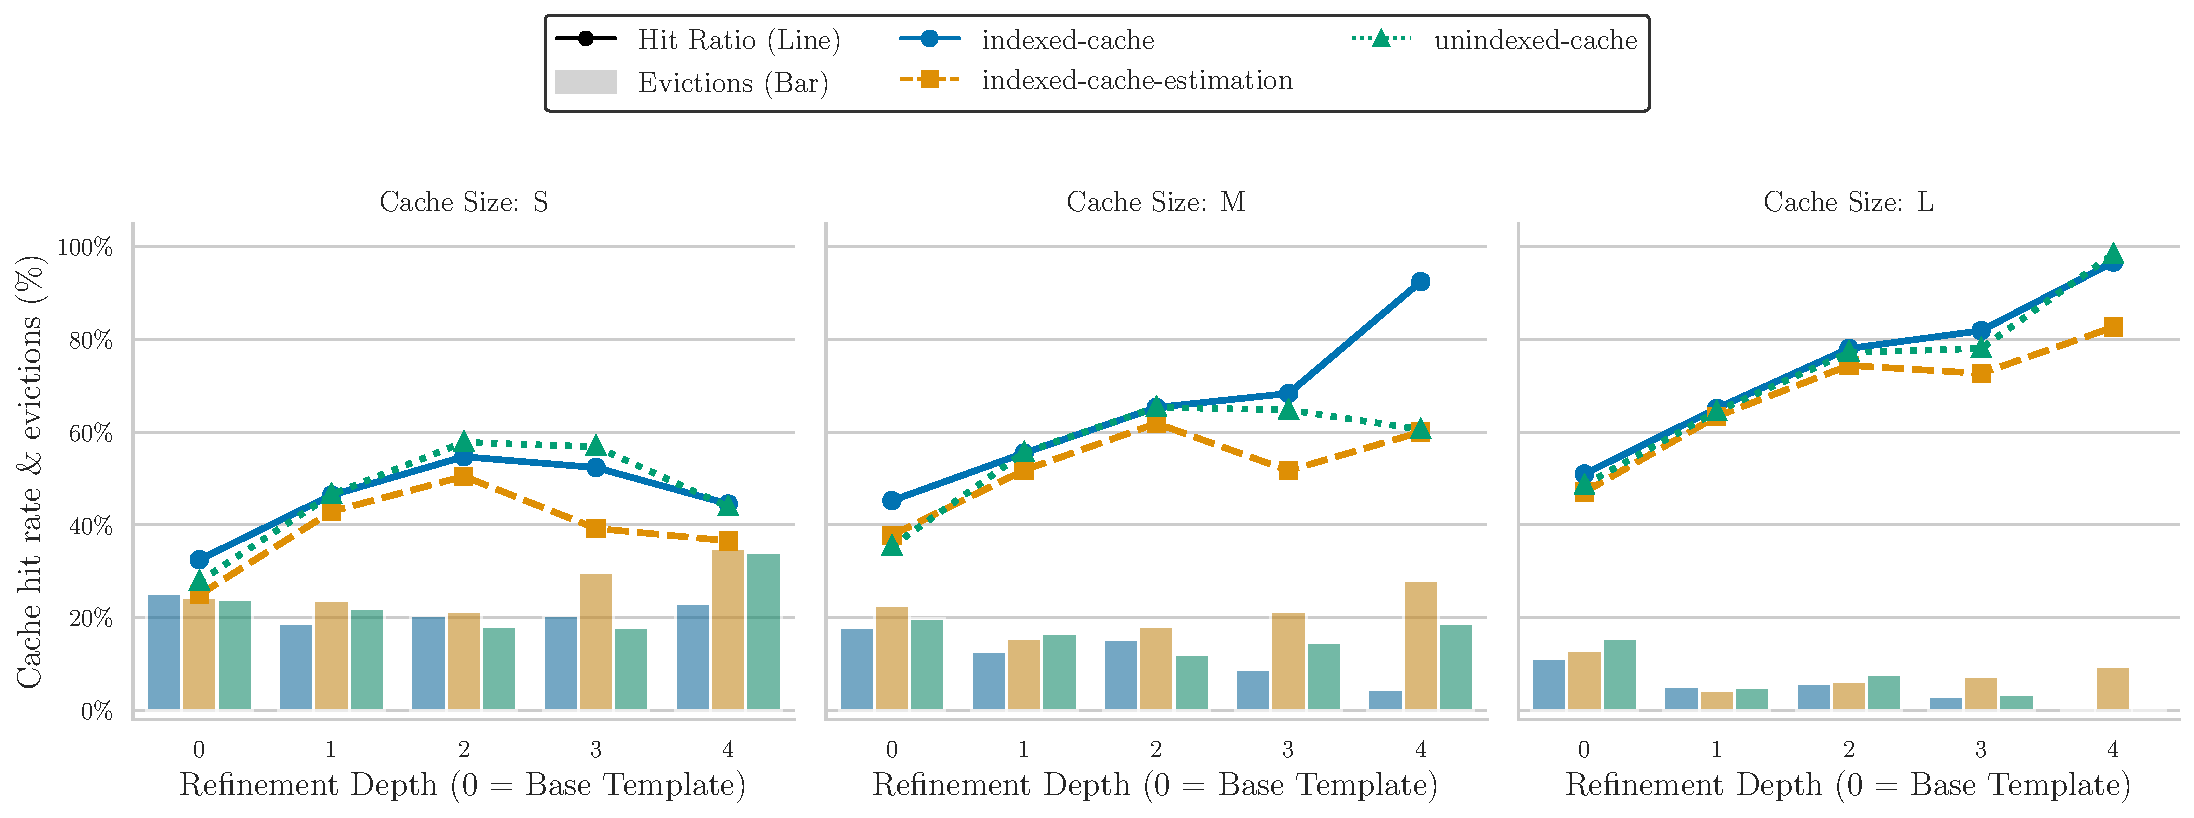
\includegraphics[width=\textwidth]{figures/combined_cache_efficiency.pdf}
%     \caption{Cache hit ratios and percentage of cache capacity evicted across refinement depths for small, medium, and large cache configurations.}
%     \label{fig:cache_efficiency}
% \end{figure*}

% At higher refinement depths, 
% performance depends heavily on cache capacity. 
% Large caches sustain high hit rates through depth 4, 
% whereas small caches experience significant thrashing,
% and degraded hit ratios. 

% Surprisingly, the indexed cache without estimation maintains high hit rates at small capacities. 
% Different caching mechanisms alter how the Node.js event loop schedules traversal and join executions,
% changing traversal order and rate.
% We suspect this variance increases temporal locality, though further analysis is needed to confirm the exact mechanism and explain why the indexed cache outperforms the unindexed baseline.

% The observed cache hit rate and eviction differences directly translate to measurable execution speedups.
% Figure 2 illustrates that the geometric mean speedup generally scales positively with refinement depth, with 
% a more pronounced effect for the throughput. 
% The indexed-cache algorithm proves particularly effective for prolonged exploratory sequences,
% achieving substantial throughput gains at depth 4 compared to the unindexed alternatives.

% \begin{figure*}[htpb]
%     \centering
%     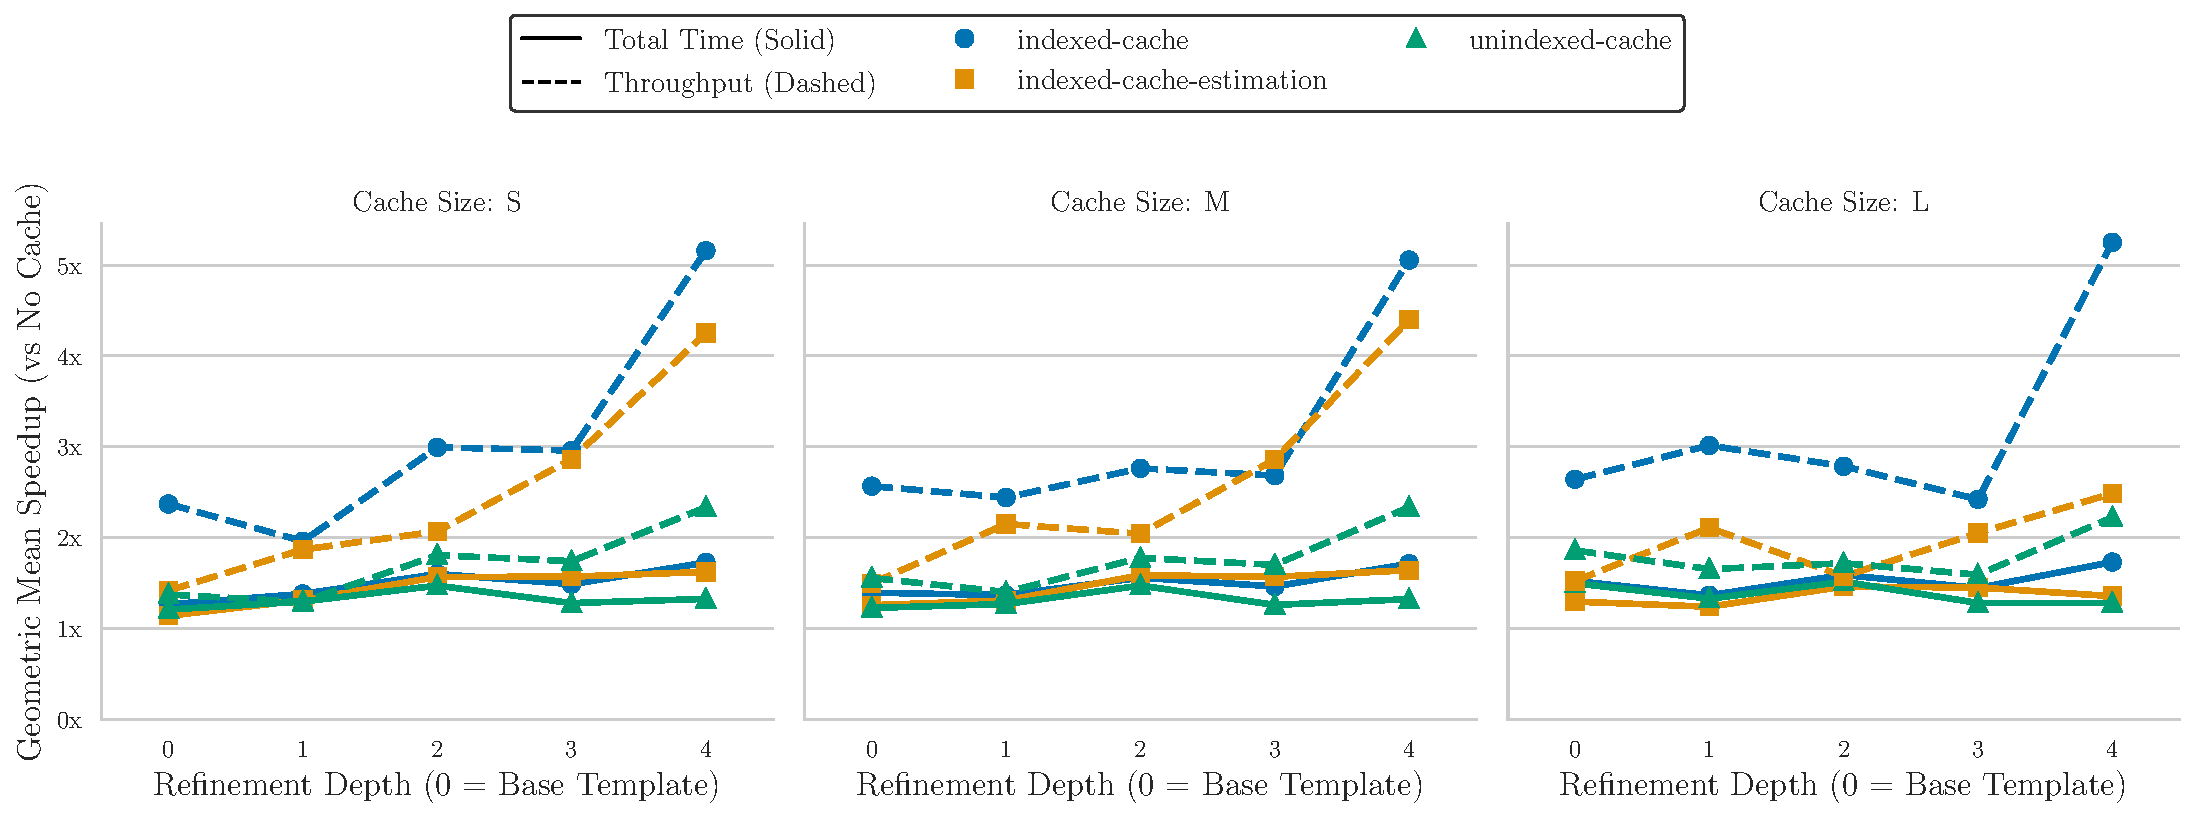
\includegraphics[width=\textwidth]{figures/temporal_throughput_line.pdf}
%     \caption{Geometric mean of observed speedups and increases respectively for total execution time and query throughput 
%     relative to the no caching baseline across refinement depths.}
%     \label{fig:temporal_throughput}
% \end{figure*}

% \subsection{Comparison To Other Evaluation Methods}

% \paragraph{Microbenchmarks-Theoretical Hit Rate Analysis}

% Cache literature extensively uses microbenchmarks of various forms 
% to analyze caching performance~\cite{nicholson2024hpcache,hartig2011caching}.
% To compare the conclusions of such a benchmark to the conclusions of the benchmark introduced in this paper
% we investigate theoretical caching speedup without management costs, 
% by executing each query template twice with simulated cache miss probabilities. 
% We excluded the estimation-based approach, 
% as using the full cache for estimation would skew the results for miss rates above zero.

% Figure~\ref{fig:theoretical_cache_performance} shows representative performance profiles for the workload. 
% Most templates (8 out of 12) show reliable improvement that scales with the hit rate for both algorithms. 
% However, certain long-running queries (e.g., interactive-discover-6, 7, and short-3) show no speedup, 
% and some even experience slowdowns. 
% These templates traverse many solid pods but do not require all traversed data. 
% We hypothesize that rapidly serving documents from an in-memory cache overwhelms the system with data, 
% slowing result production. 
% Conversely, HTTP network latency gives the JavaScript event loop time to process the join execution pipeline, 
% yielding initial results faster since only the first few requests are needed.

% \begin{figure*}[!h]
%     \centering
%     % Ensure the filename matches your generated PDF
%     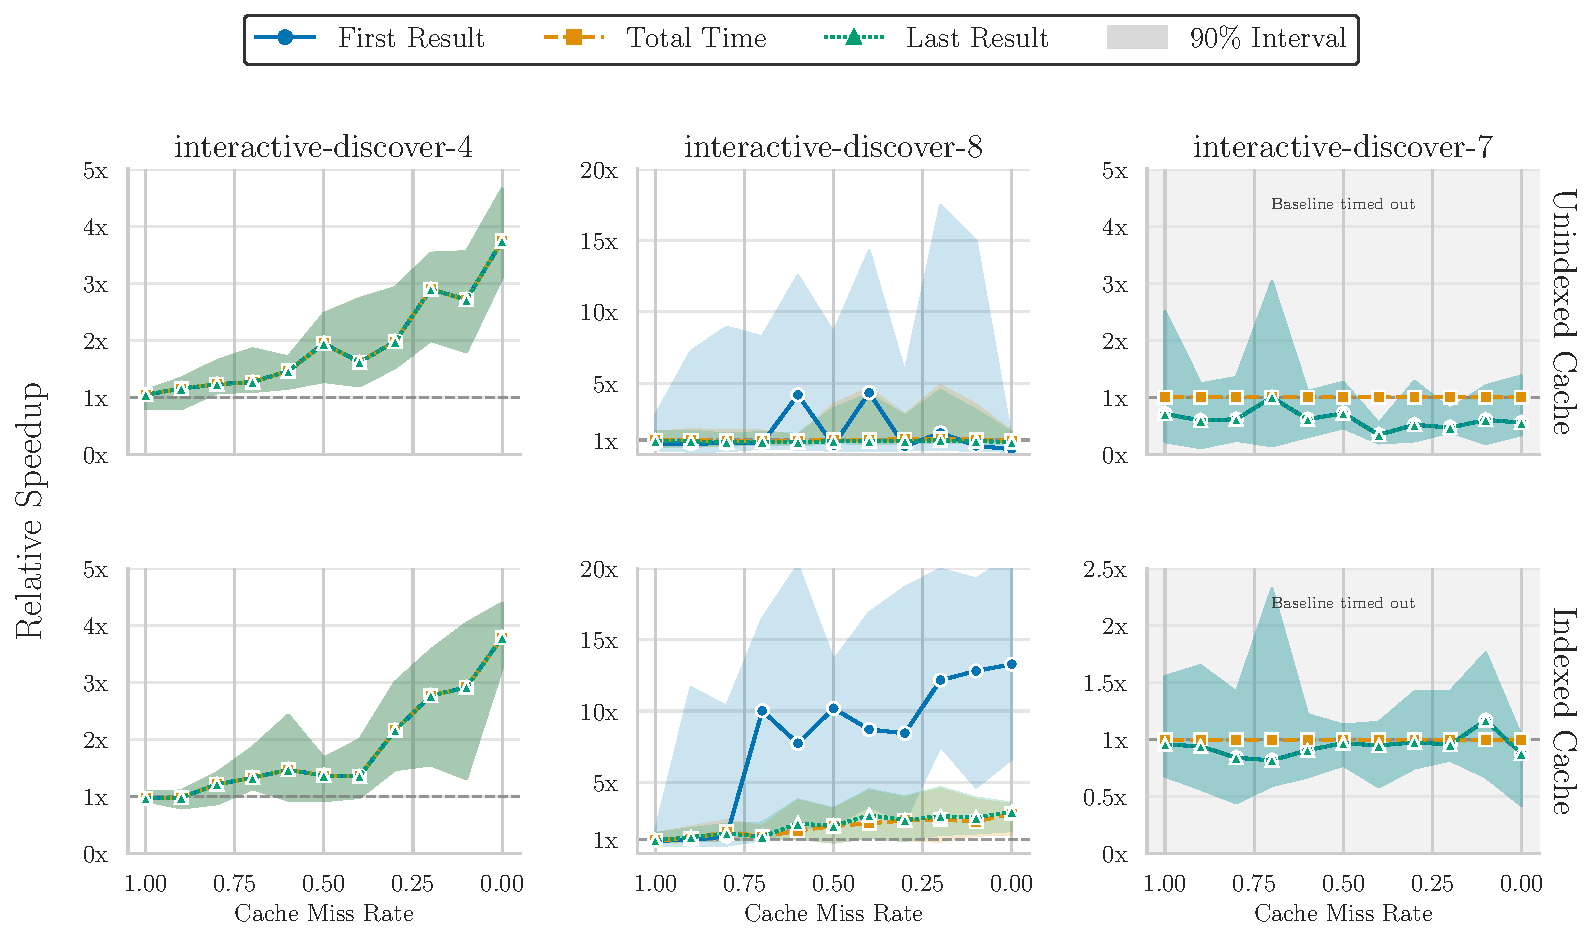
\includegraphics[width=\textwidth]{figures/synth_hit_rate_reduced.pdf}
%     \caption{ Performance of unindexed and indexed caches across representative query templates. 
%     The y-axis shows the mean speedup relative to a baseline with a 0\% hit rate.
%      Shaded regions denote the 90th percentile}
%     \label{fig:theoretical_cache_performance}
% \end{figure*}

% Both caching approaches perform similarly overall, 
% but the indexed cache significantly reduces time-to-first-result across most templates. 
% As expected, indexed caching is highly advantageous without evictions. 
% However, the initial indexing cost creates a trade-off: 
% it amplifies both speedups and slowdowns relative to an unindexed cache. 
% While this micro-benchmark approach aligns with prior literature~\cite{nicholson2024hpcache}, 
% our mixed findings show that micro-benchmarks alone fail to thoroughly evaluate client-side caching optimizations. 
% This limitation demonstrates the clear need for the comprehensive benchmark we introduce in this work.




% \paragraph{Random Query Sequences}
% Another common approach is to use random query sequences from an existing 
% benchmark~\cite{o2009star,bizer2011berlin,hartig2011caching,nicholson2024hpcache,folz2016cyclades}.
% Figure~\ref{fig:global_cache_performance_random_sequences} shows execution times 
% for sequences created by randomly grouping default SolidBench.js queries.
% For these random sequences, only large caches perform well,
% while smaller ones degrade below the baseline.
% These results misleadingly suggest that large caches are vital, 
% whereas our benchmark demonstrates significant performance benefits even with smaller sizes.
% As expected, the estimation cache performs well in both scenarios because cardinality estimation does not require cache hits.

% \begin{figure*}[htpb]
%     \centering
%     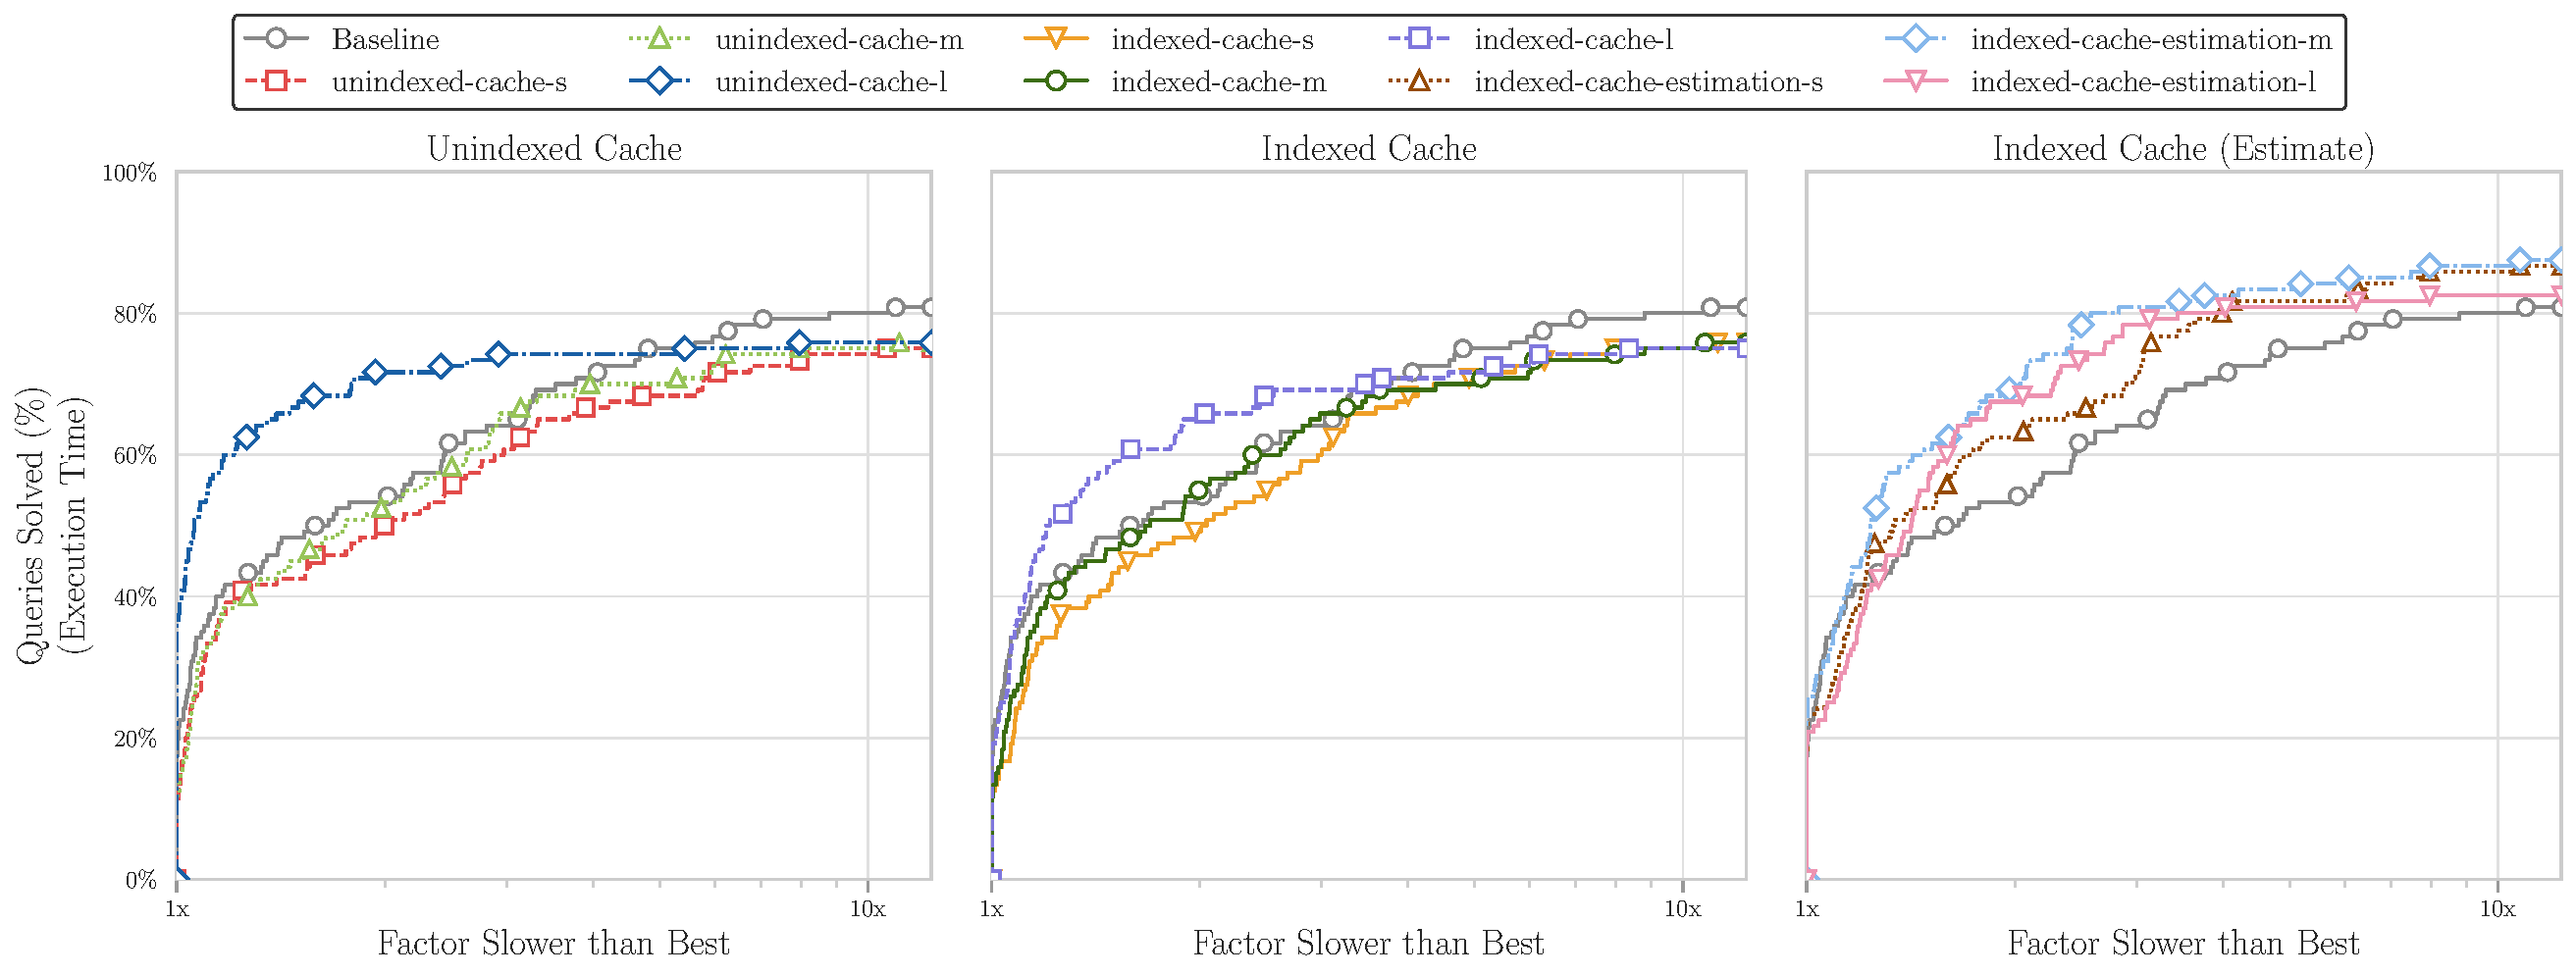
\includegraphics[width=\linewidth]{figures/performance_profile_random_sequences.pdf}
%     \caption{Performance profile of the tested cache algorithms on random query sequences.
%      The y-axis shows the percentage of queries that execute within 
%      a given performance factor (x-axis) of the fastest algorithm for that query.}
%     \label{fig:global_cache_performance_random_sequences}
% \end{figure*}

\paragraph{Scope and Limitations}
We evaluate SolidSessionBench against microbenchmarks and random sequences, 
but explicitly exclude hand-crafted scenarios and simple distributions.
Hand-crafted methods lack scalability, while simple distributions fail to capture complex user habits.
By automating logical sessions and user interests, our benchmark functions as a scalable superset of both approaches,
making direct comparison redundant. 
By contrast, the compared methods do not incorporate these sequence attributes, 
and our results show this omission risks drawing inaccurate conclusions.
\section{Conclusion}
\label{sec:conclusion}
We introduced SolidSessionBench, an evidence-based benchmark for generating realistic query sequences in decentralized environments. 
By modeling logical sessions, user interests, and iterative refinement, 
it captures client-side performance characteristics that traditional evaluation methods fail to find. 
While using Solid as the primary use case, the underlying concepts apply to approaches such as Linked Web Storage (LWS),
and we will provide an LWS-specific representation once the W3C Working Group finalizes the specifications.

Our evaluation demonstrates that traditional benchmarking methods, such as microbenchmarks and random query sequences, produce misleading estimates of real-world caching performance. 
\todo{Check if true}
By applying SolidSessionBench to caching in LTQP, we uncovered three critical insights. 
First, logical session switching severely degrades cache hit rates, proving that optimal cache sizing and eviction policies must account for session dynamics. 
Second, deep exploratory query refinement introduces significant cache invalidation challenges. 
However, it also exposes unexploited optimization opportunities, such as the 100$\times$ speedups triggered by cost-model unpredictability and cache dynamics when using disk-based caching or combining small caches with cardinality estimation.
Third, cache-based triple pattern cardinality estimation effectively optimizes link traversal queries, as previous executions provide the prior knowledge traditionally absent in LTQP.

This paper provides a clear path forward for optimizing LTQP in decentralized environments. 
Historically, the absence of prior knowledge hindered LTQP query optimization, leading to inefficient execution plans. 
Furthermore, network latency from numerous HTTP requests imposes a strict lower bound on execution times. 
Well-designed caching algorithms can address both bottlenecks simultaneously, offering a promising direction for future optimization literature.

To realize this potential and support realistic user behavior, client-side query engines must move beyond static, session-agnostic caching. 
Future research should prioritize session-aware caching mechanisms that dynamically identify and protect cross-session core entries. 
Additionally, developing intelligent cache warmup strategies and hierarchical architectures, such as combining small 
in-memory quad stores with large disk-based caches, can mitigate the performance penalties of session switching. 
Next, reverse-engineering the extreme speedup anomalies caused by inaccurate cardinality estimates could unlock
highly optimized execution plans tailored specifically for link traversal. 
Finally, future work should explore alternative cache-based cardinality estimation methods,
particularly for evaluating join cardinalities.

To ensure longevity and reuse, SolidSessionBench has been integrated into the core SolidBench ecosystem,
inheriting its established track record of community support and maintenance.
We formalize this in our sustainability plan \url{https://github.com/SolidBench/SolidBench.js/wiki/Sustainability-Plan}.
Due to the \\ seamless integration into SolidBench, its status as the standard community resource 
for evaluating decentralized query execution~\cite{eschauzier2025revisiting,vandenbrande2025incremunica,hanski2025link,tam2024opportunities}
serves as a proxy for the future adoption of this new benchmark when trying to evaluate any client-specific optimization approaches.

The framework is modular, MIT-licensed, and fully documented, with links to all code, data, 
and experiment setups available at this paper-specific hub: \url{https://github.com/RubenEschauzier/simulated-query-sequence-paper}\rt{Could you move all repos you created for this paper that are now under your personal namespace, to the KNoWS GitHub organization?}.  
This \\ extension-friendly approach to development allows researchers to easily modify or extend specific components to meet future requirements
without disrupting the broader evaluation pipeline.


\printcredits

%% Loading bibliography style file
%\bibliographystyle{model1-num-names}
\bibliographystyle{cas-model2-names}

% Loading bibliography database
\bibliography{references/bib}


%\vskip3pt

\end{document}

